\documentclass[12pt,oneside,openright,a4paper]{report}

% T1 encoding goes first so characters like < and > print properly in
% \texttt (with the old default encoding they come out as upside-down
% punctuation). It's loaded before Settings so any font packages in there
% build on top of it.
\usepackage[T1]{fontenc}

\setlength{\emergencystretch}{3em}
% -------------------------------
% Load all packages and styling
% -------------------------------
% ==============================
% ENCODING
% ==============================
\usepackage[utf8]{inputenc}
\usepackage[T1]{fontenc}

% ==============================
% PAGE LAYOUT
% ==============================
\usepackage{geometry}
\geometry{
    a4paper,
    top=2.5cm,
    bottom=2.5cm,
    left=3cm,
    right=3cm
}

\usepackage{setspace}
\onehalfspacing

% ==============================
% FONTS
% ==============================
% \usepackage[scaled]{helvet}
% \renewcommand{\familydefault}{\sfdefault}
\usepackage{lmodern}
% ==============================
% MATH & SYMBOLS
% ==============================
\usepackage{amsmath, amsthm, amsfonts}
\usepackage{siunitx}

% ==============================
% TABLES & FIGURES
% ==============================
\usepackage{graphicx}
\usepackage{subfig}
\usepackage{array}
\usepackage{makecell}
\usepackage{multirow}
\usepackage{adjustbox}
\usepackage{threeparttable}
\usepackage{tablefootnote}
\usepackage{booktabs} 

% ==============================
% CHAPTER FORMATTING
% ==============================
\usepackage{titlesec}

\titleformat{\chapter}
{\normalfont\huge\bfseries}
{\thechapter.}
{20pt}
{\huge\bfseries}

% ==============================
% NUMBERING
% ==============================
\usepackage{chngcntr}
\counterwithin{figure}{chapter}
\counterwithin{table}{chapter}

% ==============================
% BIBLIOGRAPHY
% ==============================
\usepackage{csquotes}

\usepackage[
backend=biber,
style=ieee
]{biblatex}

\addbibresource{References.bib}

% ==============================
% GLOSSARY & ACRONYMS
% ==============================
\usepackage[acronym,toc]{glossaries-extra}

% ==============================
% DIAGRAMS
% ==============================
\usepackage{tikz}

% ==============================
% COLORS
% ==============================
\usepackage{xcolor}

\definecolor{CPUTBlue}{HTML}{005696}
\definecolor{CPUTRed}{HTML}{ED1C24}

% ==============================
% PROFESSIONAL HEADERS
% ==============================
\usepackage{fancyhdr}

\setlength{\headheight}{15pt}

\pagestyle{fancy}
\fancyhf{}

\fancyhead[L]{OPS260S Operating Systems}
\fancyhead[R]{\leftmark}

\fancyfoot[C]{\thepage}

% ==============================
% PDF / LINKS
% ==============================
\usepackage{hyperref}

\hypersetup{
colorlinks=true,
linkcolor=black,
citecolor=black,
urlcolor=blue,
pdftitle={Operating Systems Group 1 Report}
}

% ==============================
% QUALITY IMPROVEMENTS
% ==============================
\usepackage{microtype}

% ==============================
% MISC
% ==============================
\usepackage{pdfpages}
\usepackage{lipsum}
\usepackage{fancyhdr}
\setlength{\headheight}{28pt}

% Figure packages. subcaption/subfigure are deliberately NOT used any more:
% every screenshot is its own figure, which avoids the subfigure errors and
% keeps each image sitting exactly where it appears in the text.
\usepackage{graphicx}      % \includegraphics
\usepackage{float}         % [H] = "put it right here"
\usepackage[section]{placeins} % floats can never drift past the end of a section

% \screenshot{file}{caption}{label}
% One image per figure, placed exactly where it is written ([H]). The height
% limit is there so two screenshots fit on a page and a tall image can never
% overflow it; keepaspectratio stops the image being stretched to fit.
\newcommand{\screenshot}[3]{%
    \begin{figure}[H]
        \centering
        \includegraphics[width=0.85\textwidth,height=0.35\textheight,keepaspectratio]{#1}
        \caption{#2}
        \label{#3}
    \end{figure}%
}

% -------------------------------
% GLOSSARIES
% -------------------------------


% --- CPUT REPORT INFORMATION ---
\newcommand*{\getUniversity}{Cape Peninsula University of Technology}
\newcommand*{\getFaculty}{Faculty of Engineering and the Built Environment}
\newcommand*{\getDepartment}{Department of Electrical, Electronic, and Computer Engineering}

\newcommand*{\getTitle}{%
\fontsize{16pt}{18pt}\selectfont\bfseries
Design and Implementation of a Secure Windows Server 2019 Infrastructure for Enterprise Network Services\\[0.4em]
}

\newcommand*{\getAuthor}{Group 1}

% Degree Information
\newcommand*{\getDoctype}{Group project report submitted in partial fulfilment of the requirements for the degree}
\newcommand*{\getDegree}{Bachelor of Engineering Technology in Computer Engineering}

\newcommand*{\getSupervisor}{Mr. Vusumuzi Moyo}
\newcommand*{\getCoSupervisor}{Mr. Adrian Wyngaard}
\newcommand*{\getCourseCode}{OPS260S - OPERATING SYSTEMS 2}

\newcommand*{\getCampus}{Bellville Campus}
\newcommand*{\getSubmissionDate}{September 2026}

% Copyright
\newcommand*{\getCopyright}{
The report may not be published either in part 
(in scholarly, scientific or technical journals), or as a whole 
(as a monograph), unless permission has been obtained from the University.
}

% =================================================
% DOCUMENT START
% =================================================
\begin{document}

% -------------------------------
% FRONT MATTER
% -------------------------------
\pagenumbering{roman}

\begin{titlepage}
    \begin{center}

        % --- Header block: logo + institution ---
        \IfFileExists{Images/logo_CPUT.png}{%
            
\includegraphics[height=25mm]{Images/logo_CPUT.png}
        }{%
            \vspace*{25mm}
        }

        \vspace{4mm}
        {\large \scshape Department of Electrical, Electronic and Computer Engineering\par}

        \vfill

        % --- Title block ---
        \rule{0.8\textwidth}{0.4pt}\\[6mm]
        {\huge \bfseries \getTitle \par}
        \vspace{3mm}
        \rule{0.8\textwidth}{0.4pt}

        \vspace{12mm}

        {\Large by}\\[4mm]
        {\Large \bfseries \getAuthor}

        \vfill

        % --- Degree statement ---
        {\large \getDoctype}\\[0.4cm]
        {\large \bfseries \getDegree}\\[0.4cm]
        {\large in the \getFaculty}\\[0.4cm]
        {\large at the \getUniversity}

        \vfill

        % --- Examiner / course info ---
        \begin{tabular}{r l}
            Examiner:    & \getSupervisor \\
            Course Code: & \getCourseCode \\
            % \ifx\getCoSupervisor\empty \else Co-supervisor: & \getCoSupervisor \\ \fi
        \end{tabular}

        \vspace{10mm}

        {\large \getCampus}\\
        {\large \getSubmissionDate}

        \vfill

        % --- Copyright statement ---
        \begin{minipage}{0.8\textwidth}
            \centering
            \footnotesize \getCopyright
        \end{minipage}

    \end{center}
\end{titlepage}

\setcounter{page}{1}

\chapter*{Declaration of Authorship}

We, the undersigned, declare that the contents of this report represent our own unaided work, except where explicitly acknowledged. The report has not previously been submitted for academic examination towards any qualification. Furthermore, it represents our own opinions and not necessarily those of the Cape Peninsula University of Technology.

\vspace{20mm}

\begin{tabular}{@{}p{6.2cm} p{6.2cm}@{}}
\parbox{6.2cm}{\centering
\includegraphics[width=4.8cm,height=1.6cm]{Images/signature_anh_duy_nguyen}} & 
\parbox{6.2cm}{\centering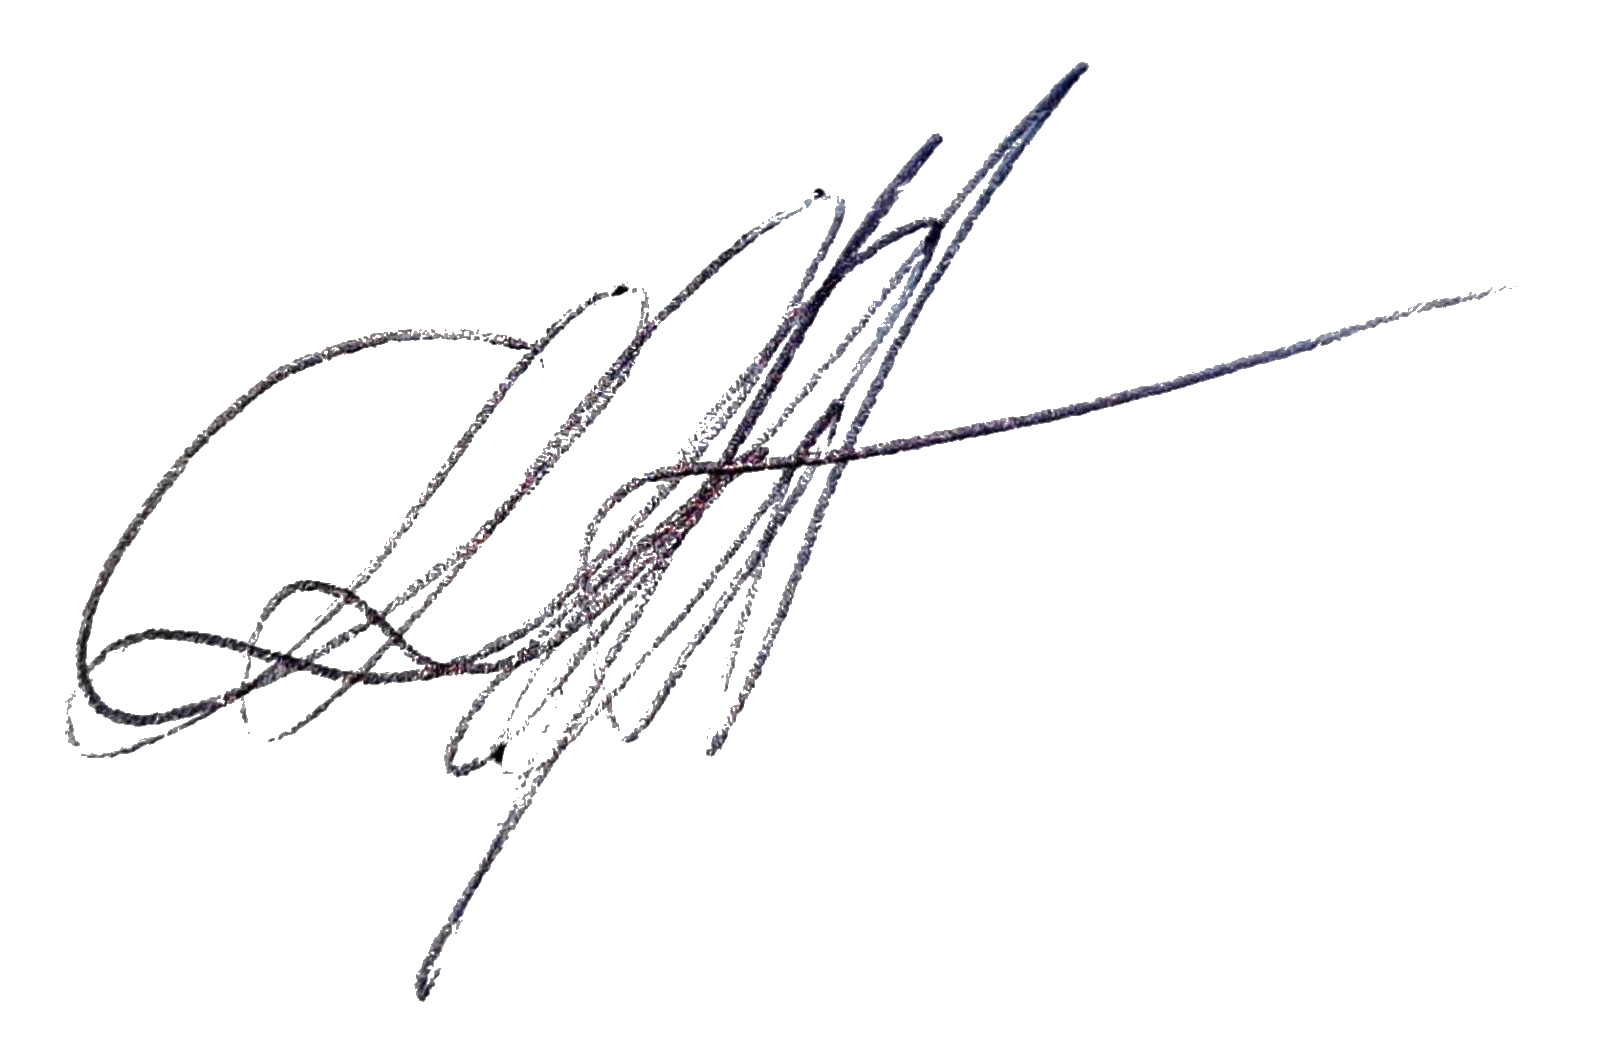
\includegraphics[width=4.8cm,height=1.6cm]{Images/signature_carl_lamprecht}} \\
\rule{6.2cm}{0.4pt} & \rule{6.2cm}{0.4pt} \\
Anh Duy Nguyen, 251163733 & Carl Lamprecht, 205133681 \\[6mm]

\parbox{6.2cm}{\centering
\includegraphics[width=4.8cm,height=1.6cm]{Images/signature_peter_ngesi}} & 
\parbox{6.2cm}{\centering
\includegraphics[width=4.8cm,height=1.6cm]{Images/signature_gian_koekemoer}} \\
\rule{6.2cm}{0.4pt} & \rule{6.2cm}{0.4pt} \\
Peter Hlalubonga Ngesi, 250281228 & Gian Koekemoer, 250060248 \\[6mm]

\parbox{6.2cm}{\centering
\includegraphics[width=4.8cm,height=1.6cm]{Images/signature_tihmo_koch}} & 
\parbox{6.2cm}{\centering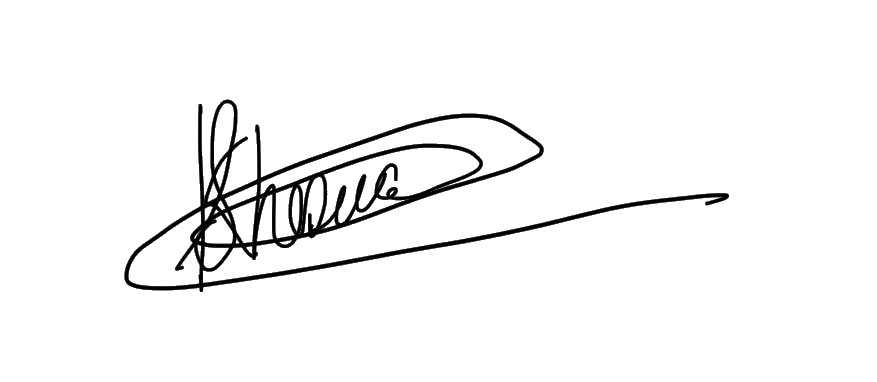
\includegraphics[width=4.8cm,height=1.6cm]{Images/signature_sibusiso_kheswa}} \\
\rule{6.2cm}{0.4pt} & \rule{6.2cm}{0.4pt} \\
Tihmo Koch, 250030993 & Sibusiso Isaac Kheswa, 250175282 \\[6mm]

\today \\[1mm]
\rule{6.2cm}{0.4pt} \\
\footnotesize Date 
\end{tabular}

\vspace{10mm}

% ==================== AI Declaration (Half Size Signatures) ====================

\chapter*{AI Declaration}

We declare that generative artificial intelligence (AI) tools were used in the preparation of this report as follows:

\begin{itemize}
    \item \textbf{Grammar, spelling, and language refinement} (e.g., rephrasing for clarity and readability).
    \item \textbf{LaTeX formatting assistance} (structure and code improvements).
\end{itemize}

All AI-generated suggestions were carefully reviewed, edited, and verified by the authors. The core ideas, analysis, research, and final content are entirely the work of the authors. No AI tool was used to generate original ideas, conduct the literature review, or produce the main technical content without substantial human input and oversight.

This declaration is made in accordance with academic integrity principles and the Cape Peninsula University of Technology guidelines on responsible AI use.

\vspace{10mm}

\begin{tabular}{@{}p{6.2cm} p{6.2cm}@{}}
\parbox{6.2cm}{\centering
\includegraphics[width=2.3cm,height=0.8cm]{Images/signature_anh_duy_nguyen}} & 
\parbox{6.2cm}{\centering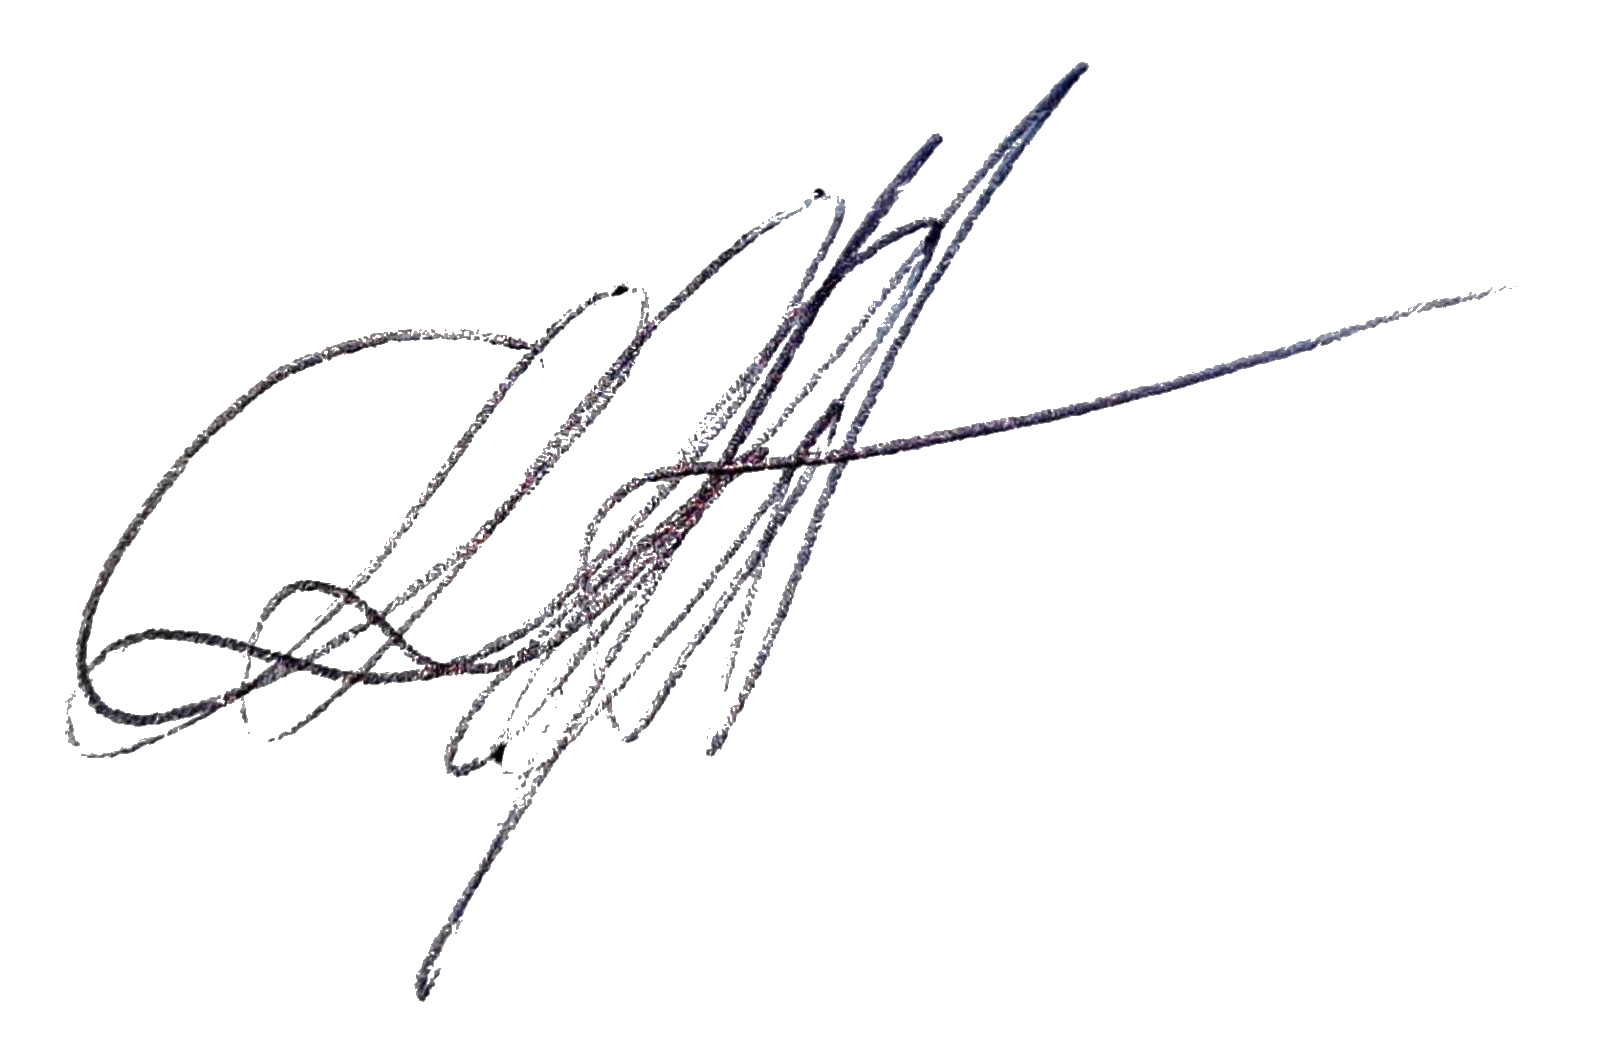
\includegraphics[width=2.3cm,height=0.8cm]{Images/signature_carl_lamprecht}} \\
\rule{6.2cm}{0.4pt} & \rule{6.2cm}{0.4pt} \\
Anh Duy Nguyen, 251163733 & Carl Lamprecht, 205133681 \\[4mm]

\parbox{6.2cm}{\centering
\includegraphics[width=2.3cm,height=0.8cm]{Images/signature_peter_ngesi}} & 
\parbox{6.2cm}{\centering
\includegraphics[width=2.3cm,height=0.8cm]{Images/signature_gian_koekemoer}} \\
\rule{6.2cm}{0.4pt} & \rule{6.2cm}{0.4pt} \\
Peter Hlalubonga Ngesi, 250281228 & Gian Koekemoer, 250060248 \\[4mm]

\parbox{6.2cm}{\centering
\includegraphics[width=2.3cm,height=0.8cm]{Images/signature_tihmo_koch}} & 
\parbox{6.2cm}{\centering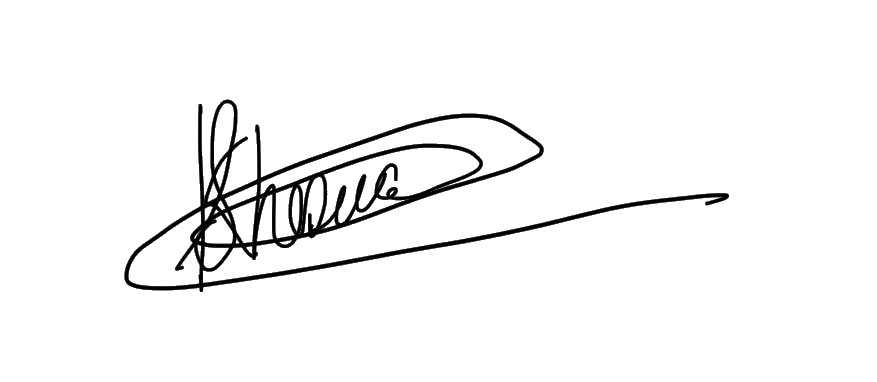
\includegraphics[width=2.3cm,height=0.8cm]{Images/signature_sibusiso_kheswa}} \\
\rule{6.2cm}{0.4pt} & \rule{6.2cm}{0.4pt} \\
Tihmo Koch, 250030993 & Sibusiso Isaac Kheswa, 250175282 \\[4mm]

\today \\[1mm]
\rule{6.2cm}{0.4pt} \\
\footnotesize Date 
\end{tabular}
\chapter*{Abstract}

\lipsum

\vspace{5mm}
\textbf{Keywords:} Operating Systems, Kernel Architecture, Resource Utilization, Performance Optimization, Memory Management, Linux, Windows

\clearpage
\tableofcontents

\clearpage
\addcontentsline{toc}{chapter}{List of Figures}
\listoffigures

\clearpage
\addcontentsline{toc}{chapter}{List of Tables}
\listoftables

% -------------------------------
% GLOSSARY & ACRONYMS
% -------------------------------
% -------------------------------
% MAIN MATTER
% -------------------------------
\clearpage
\pagenumbering{arabic}
\setcounter{page}{1}

\chapter{Introduction}

\lipsum

\section{Background}

\lipsum

\section{Objectives}

The objectives of this report are:
\lipsum

\section{Report Structure}

The remainder of this report is organised as follows:
\lipsum
\chapter{Installation and Initial Configuration of Windows Server 2019}

\section{Introduction}

This chapter describes the installation and initial configuration of Windows Server 2019 within the virtualised environment used during Semester 1. The purpose of this stage was to establish a functioning server that could support the deployment of the network services required for the project.

The installation process involved preparing the virtual machine using VirtualBox, installing the operating system, and completing the initial server configuration. These steps provided the foundation for the subsequent configuration of Active Directory Domain Services (AD DS), DNS, DHCP, Group Policy, Remote Access, and Windows Certificate Services.

\section{Virtual Machine Preparation}

Before installing Windows Server 2019, a virtual machine was prepared using VirtualBox. Virtualisation allows multiple operating systems to run on a single physical computer while maintaining separate virtual environments.

The virtual machine was configured with the necessary resources to support the operating system and the planned server roles. These resources included virtual memory, processor allocation, virtual storage, and a network adapter. The Windows Server 2019 installation media was then attached to the virtual machine, allowing it to boot from the installation image.

% Virtual machine configuration screenshots, in the order the steps were done.
% \screenshot{image}{caption}{label} is defined in Main.tex.
\screenshot{Images/VM/VM_install_01.png}{Initial Virtual Machine Configuration.}{fig:vm_configuration1}
\screenshot{Images/VM/VM_install_02.png}{Virtual Machine Configuration Step 2.}{fig:vm_configuration2}
\screenshot{Images/VM/VM_install_03.png}{Virtual Machine Configuration Step 3.}{fig:vm_configuration3}
\screenshot{Images/VM/VM_install_04.png}{Virtual Machine Configuration Step 4.}{fig:vm_configuration4}
\screenshot{Images/VM/VM_install_05.png}{Virtual Machine Configuration Step 5.}{fig:vm_configuration5}
\screenshot{Images/VM/VM_install_06.png}{Final Virtual Machine Configuration Step.}{fig:vm_configuration6}

\section{Installation of Windows Server 2019}

Once the virtual machine had been configured, it was started and the Windows Server 2019 installation process was initiated. The installation wizard was used to select the appropriate language, time and currency format, and keyboard layout.

The required Windows Server 2019 edition was then selected. The installation proceeded by accepting the applicable licence terms, selecting the installation type, and choosing the virtual disk on which the operating system would be installed.

After the installation files had been copied and the required setup operations completed, the virtual machine restarted. The initial administrator password was configured, allowing access to the server using the local Administrator account.

% Windows Server installation screenshots, in installation order.
\screenshot{Images/WinServ_install/WinServer_install_01.png}{Installation Screen 1.}{fig:server_installation1}
\screenshot{Images/WinServ_install/WinServer_install_02.png}{Installation Screen 2.}{fig:server_installation2}
\screenshot{Images/WinServ_install/WinServer_install_03.png}{Installation Screen 3.}{fig:server_installation3}
\screenshot{Images/WinServ_install/WinServer_install_04.png}{Installation Screen 4.}{fig:server_installation4}
\screenshot{Images/WinServ_install/WinServer_install_05.png}{Installation Screen 5.}{fig:server_installation5}
\screenshot{Images/WinServ_install/WinServer_install_06.png}{Installation Screen 6.}{fig:server_installation6}
\screenshot{Images/WinServ_install/WinServer_install_07.png}{Installation Screen 7.}{fig:server_installation7}
\screenshot{Images/WinServ_install/WinServer_install_08.png}{Installation Screen 8.}{fig:server_installation8}
\screenshot{Images/WinServ_install/WinServer_install_09.png}{Windows Server Account Set-Up.}{fig:server_installation9}
\screenshot{Images/WinServ_install/WinServer_install_10.png}{Windows Server Log-In Screen.}{fig:server_installation10}
\screenshot{Images/WinServ_install/WinServer_install_11.png}{Windows Server Loaded and installed.}{fig:server_installation11}

\section{Testing}

Testing was conducted to verify that Windows Server 2019 had been installed successfully and that the initial server configuration was functioning as expected. The tests focused on operating system availability, server identification, network configuration, and basic network connectivity.

\subsection{Operating System Verification}

The server was restarted to confirm that Windows Server 2019 could boot successfully after installation. The administrator was able to log in, and the Server Manager dashboard was accessible. This confirmed that the operating system was operational and ready for further configuration.

\screenshot{Images/WinServ_install/WinServer_dash_01.png}{Server Manager dashboard following the installation of Windows Server 2019.}{fig:server_dashboard}

The dashboard provided access to the server's management tools and the interface used to install and configure additional server roles and features.

Further testing should verify the server hostname, IP configuration, and network connectivity. The following commands can be used to perform these checks:

\begin{itemize}
    \item \texttt{hostname} -- displays the configured computer name.
    \item \texttt{ipconfig /all} -- displays the network adapter configuration.
    % \textless and \textgreater are used because a bare < or > prints as upside-down
    % punctuation in text mode unless T1 font encoding is loaded.
    \item \texttt{ping \textless{}gateway-IP\textgreater{}} -- tests connectivity to the configured network gateway, where applicable.
\end{itemize}

The outputs should be recorded and included as supporting evidence. Any failed tests should be investigated and resolved before proceeding with the configuration of additional server roles.

More comprehensive testing of Active Directory Domain Services, DNS, DHCP, Remote Access, and Windows Certificate Services is addressed in the relevant chapters of this report.

\section{Chapter Summary}

This chapter described the preparation of the virtual machine, installation of Windows Server 2019, and completion of the initial server configuration. The process established the operating system environment required for the deployment of additional server roles and network services.

Initial verification procedures were also described to assess operating system availability, server identification, network configuration, and connectivity. These steps establish the foundation for the remaining stages of the project.

The next chapter discusses the configuration and testing of Active Directory Domain Services (AD DS), which provides centralised management of users, computers, and authentication within the network environment.
\include{Chapters/Chapter3_ADDS}
\chapter{DHCP Configuration}

\section{Background}
\paragraph{}
Every machine, from computers to servers, requires an IP address
for it to be able to send and receive packets of data or information. (\cite{masterWS19})
These IP addresses act like home addresses on a street, and whilst DNS is 
responsible for resolving those IP addresses into names, there are two ways 
of assigning IP addresses to machines. These methods are static addressing
and DHCP (\cite{masterWS19}).

\paragraph{}
Static Addressing is the process of configuring IP addresses on a system
manually. It is a hands-on approach where IP addresses
are physically plugged into the NIC settings on a particular device (\cite{masterWS19}).
Despite its simplicity, this method is not scalable in environments that host
multiple devices like a small or large company, where there are laptops, desktops, 
printers, servers or other types of machines (\cite{masterWS19}). Each of these
devices needs an IP address, however manually assign them becomes tedious at a larger scale. The solution
to this problem lies in the Dynamic Host Configuration Protocol (DHCP) (\cite{masterWS19}).

\paragraph{}
DHCP is a protocol that solves the problem of providing IP addresses for many devices
on a wide scale. It allows for machines or devices that are plugged into the network and obtain 
IP address information (\cite{masterWS19}). This ability to assign IP address information to devices 
allows for DHCP to have multiple applications. When a laptop or phone is connected to a Wi-Fi router
to gain internet access, a DHCP server allows for that device to route traffic on the network by assigning
IP addressing information (\cite{masterWS19}). When a device connects to public Wi-Fi, its DHCP server runs on the router itself
and in businesses where Windows Server serves as a datacenter, DHCP services are most often hosted 
on one or more servers across the network (\cite{masterWS19}).

\section{Configuration Steps}
\subsection{DHCP Post-Install configuration}
Like other roles, the DHCP server needs to be provided a role during the 
installation phase. After the DHCP role has been added to the server, 
it isn't yet properly configured. 

\paragraph{}
The DHCP server can give clients two kinds of access groups: DHCP Administrators and DHCP Users (\cite{DHCPgroups}).
DHCP Users have read-only access to the server, which allows them to view, but not to modify server data, including DHCP server 
configuration, registry keys, DHCP log files, and the database (\cite{DHCPgroups}). They cannot create scopes, modify options values, create 
reservations or exclusion ranges, and more.
DHCP Administrators are able to view and modify data at the DHCP server (\cite{DHCPgroups}). They can 
create and delete scopes, add reservations, change option values, create superscopes or perform
 any other activity needed to adminster the DHCP server (\cite{DHCPgroups}). Despite this overseering control, they do not 
have unlimited administrative rights,because they on have rights on the local computer only (\cite{DHCPgroups}). 

\paragraph{}
These two groups are local to the server as well, meaning they cannot authorize DHCP Servers. 
This can only be done by Domain Admins(\cite{DHCPgroups}). Authorizing the server is needed because DHCP communication typically occurs before any user
or computer authentiation. DHCP protocols are based on IP protocols as well, therefore, an unknown DHCP server could 
provide invalid information to clients. Authorization prevents this (\cite{DHCPauthor}).

\paragraph{}
The authorization of the DHCP server in the wizard required for users to be 
given credentials that they would need to access the server on a user level. So far the only 
credential set was \texttt{OPS\textbackslash{}Administrator}.For any users who attempt to 
connect to the server in future, they must use this username. 

\begin{figure}[H]
    \centering
    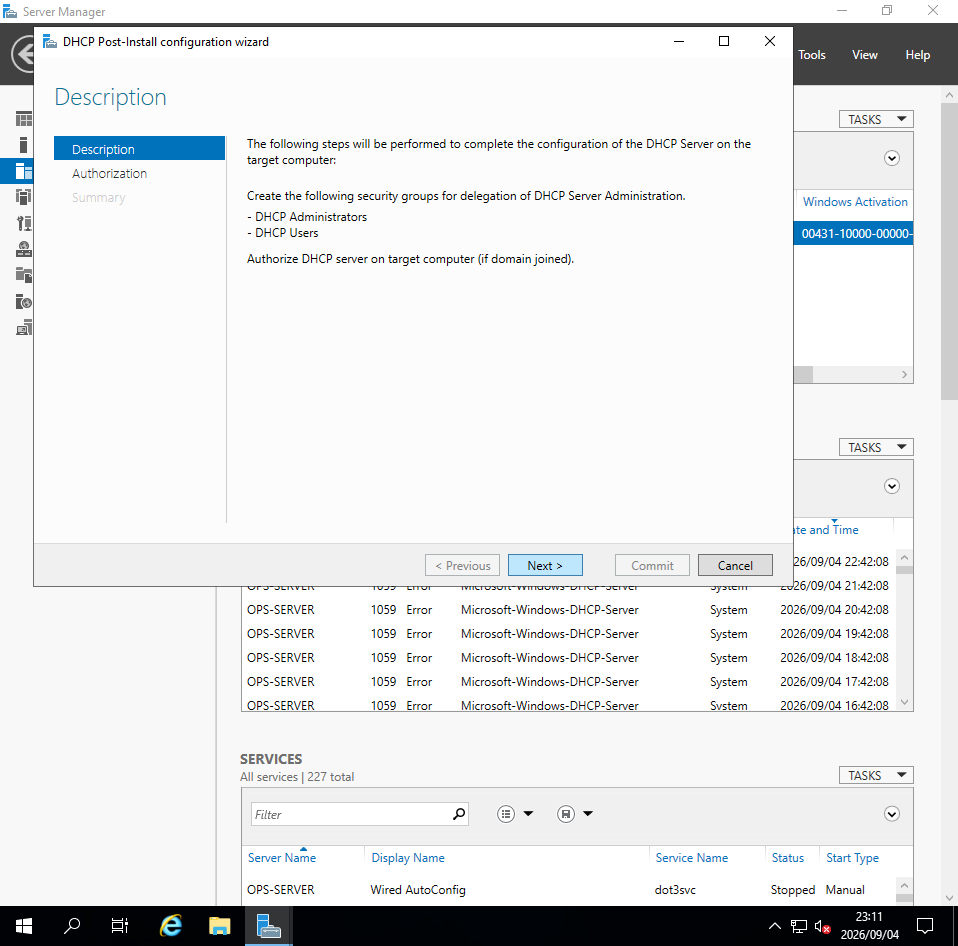
\includegraphics[width=0.7\linewidth]{Images/DHCP/DHCP_01.png}
    \caption{Description of DHCP Post-Install Configuration Wizard}
\end{figure}

\begin{figure}[H]
    \centering
    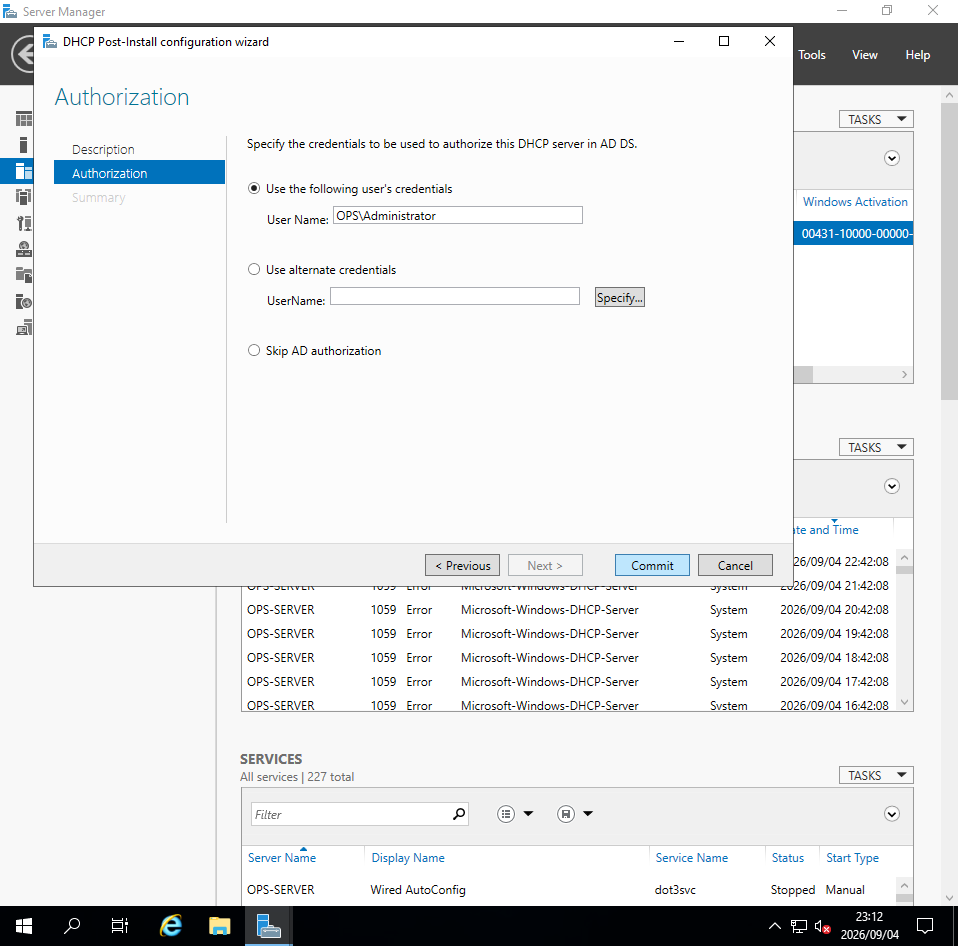
\includegraphics[width=0.7\linewidth]{Images/DHCP/DHCP_02.png}
    \caption{Authorization of DHCP Post-Install Configuration Wizard}
\end{figure}

\begin{figure}[H]
    \centering
    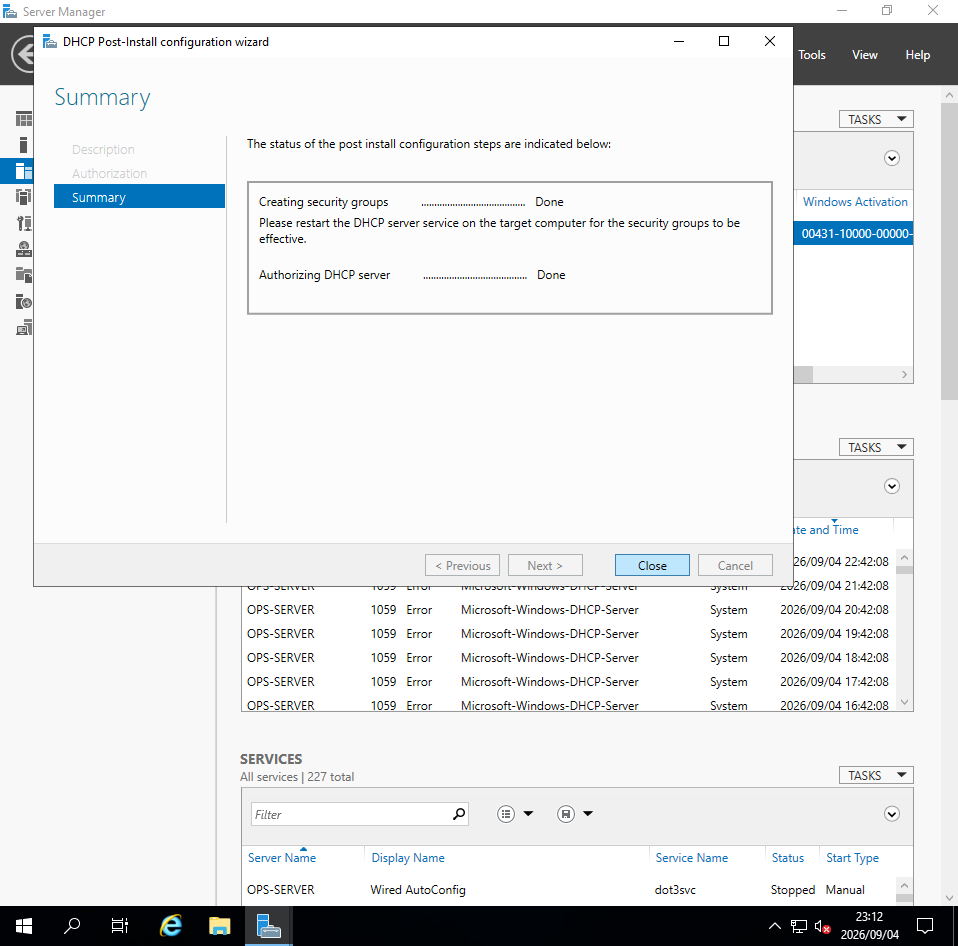
\includegraphics[width=0.7\linewidth]{Images/DHCP/DHCP_03.png}
    \caption{Post Install Configuration Completed}
\end{figure}

\subsection{The DHCP Scope}
\paragraph{}
For a DHCP server to hand out IP addresses, it needs to know IP addresses,
subnet mask, default gateway and DNS server addresses are within the network so that it can 
package and hand out the information to computers who request it. This package of information 
is called a DHCP scope (\cite{masterWS19}).

\paragraph{}
To begin defining the scope, we decided to launch a management tool using the Tools menu 
inside the Server Manager. This will open up a window for DHCP with the name of the device 
that the server is located on.

\begin{figure}[H]
    \centering
    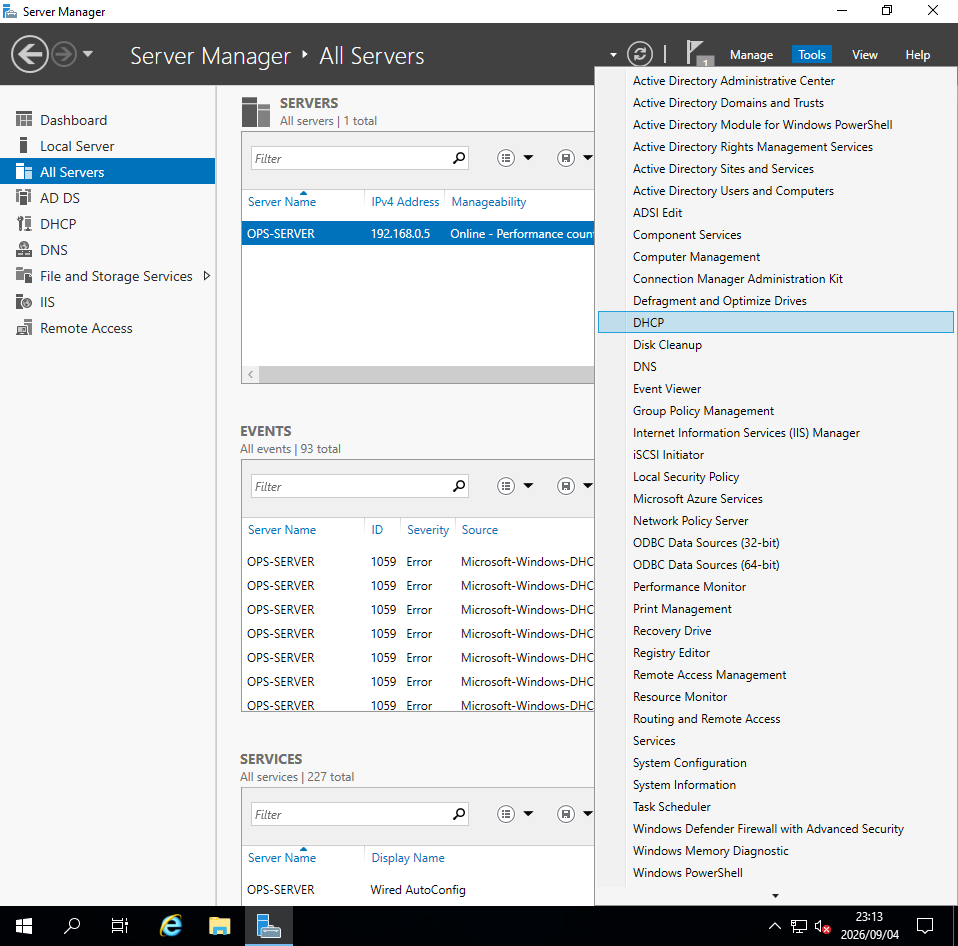
\includegraphics[width=0.7\linewidth]{Images/DHCP/DHCP_04.png}\
    \caption{DHCP Selected on Tools Dropdown Menu}
\end{figure}

\begin{figure}[H]
    \centering
    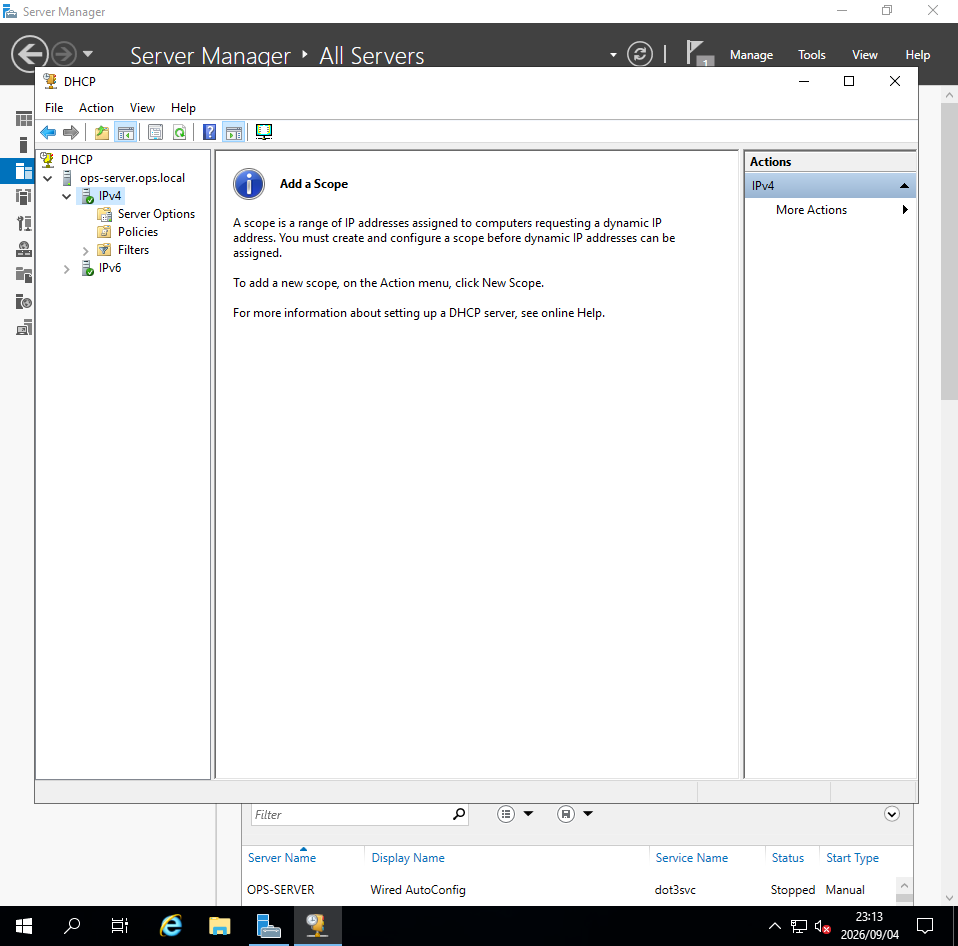
\includegraphics[width=0.7\linewidth]{Images/DHCP/DHCP_05.png}
    \caption{DHCP Windows}
\end{figure}
%two figures

\paragraph{}
After opening the DHCP window, the computer was selected and dropped down two protocols: IPv4 and IPv6.
The former was selected and first left-clicked on, where it gave information regarding the addition of a scope, along with the server 
options, policies and filters. This protocol did not have a scope as yet, so it needed to be configured.
To properly begin the process, IPv4 was right-clicked on, giving a drop-down menu when the option to add 
a new scope was present. Choosing this option opened the New Scope Wizard. After clicking next on the wizard, the basics 
of the scope needed to be decided. The name given was GROUP 1-SCOPE.

\begin{figure}[H]
    \centering
    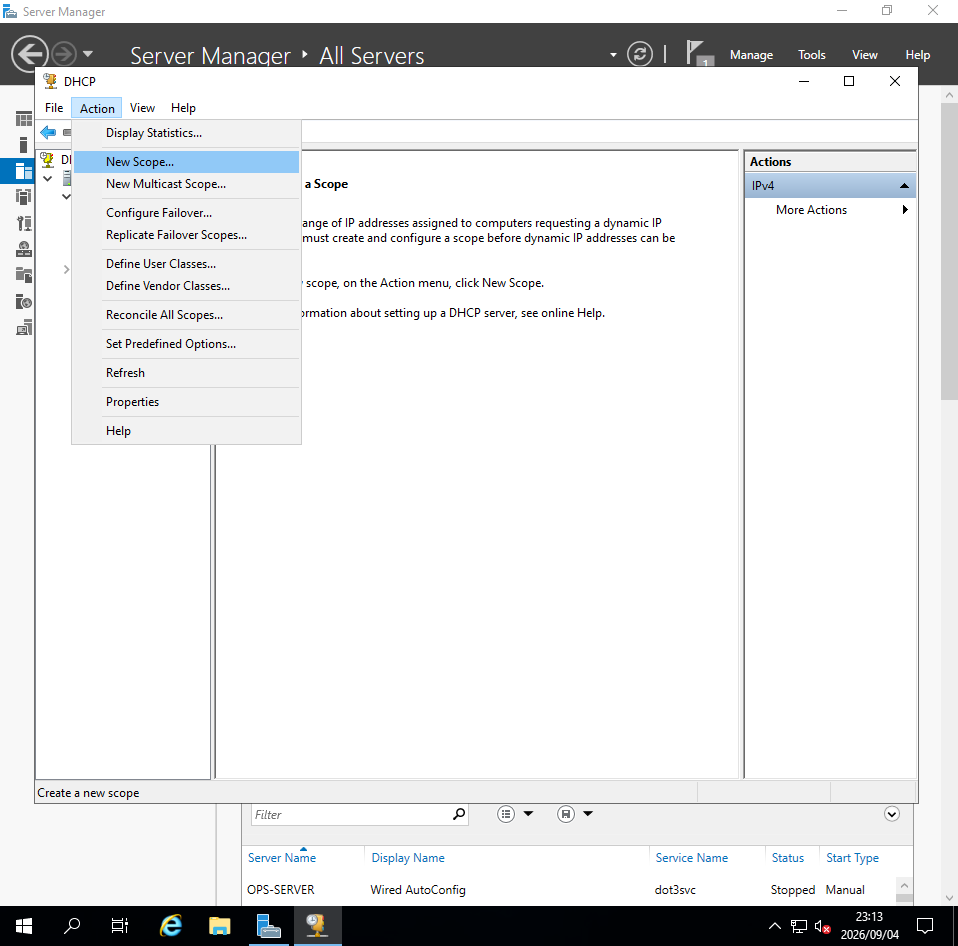
\includegraphics[width=0.7\linewidth]{Images/DHCP/DHCP_06.png}
    \caption{Adding a Scope}
\end{figure}
\begin{figure}[H]
    \centering
    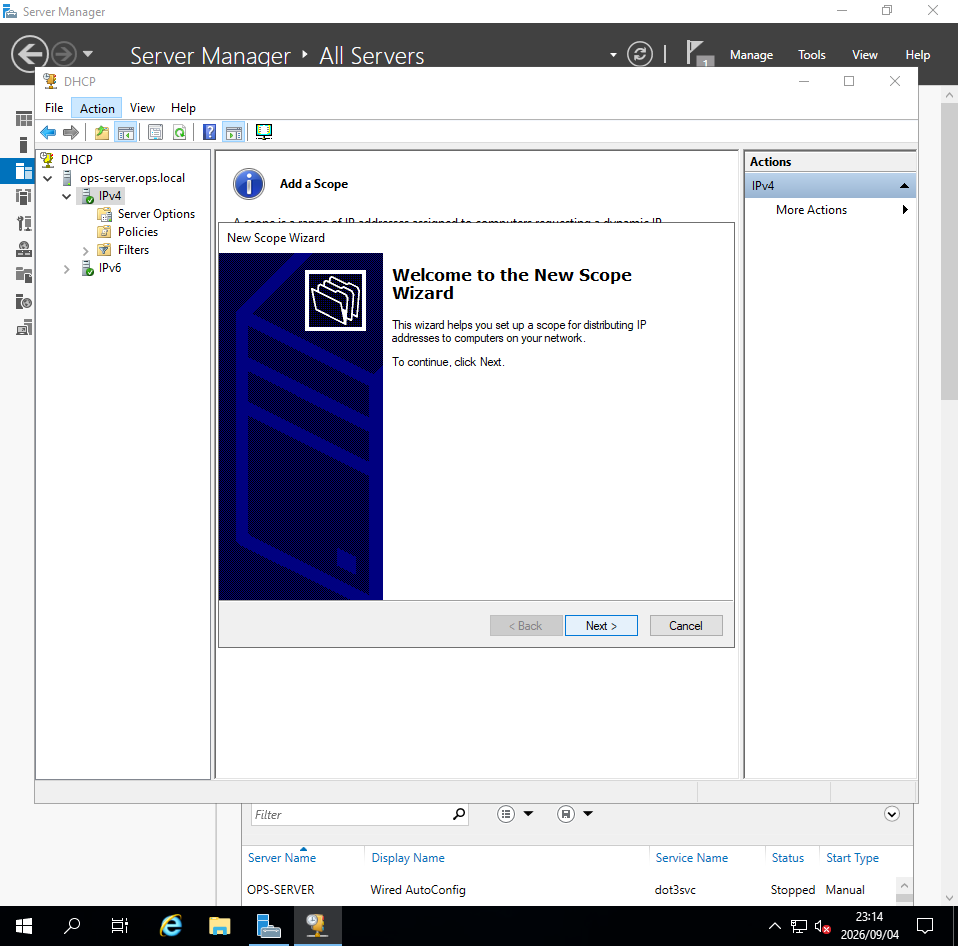
\includegraphics[width=0.7\linewidth]{Images/DHCP/DHCP_07.png}
    \caption{New Scope Wizard}
\end{figure}

\begin{figure}[H]
    \centering
    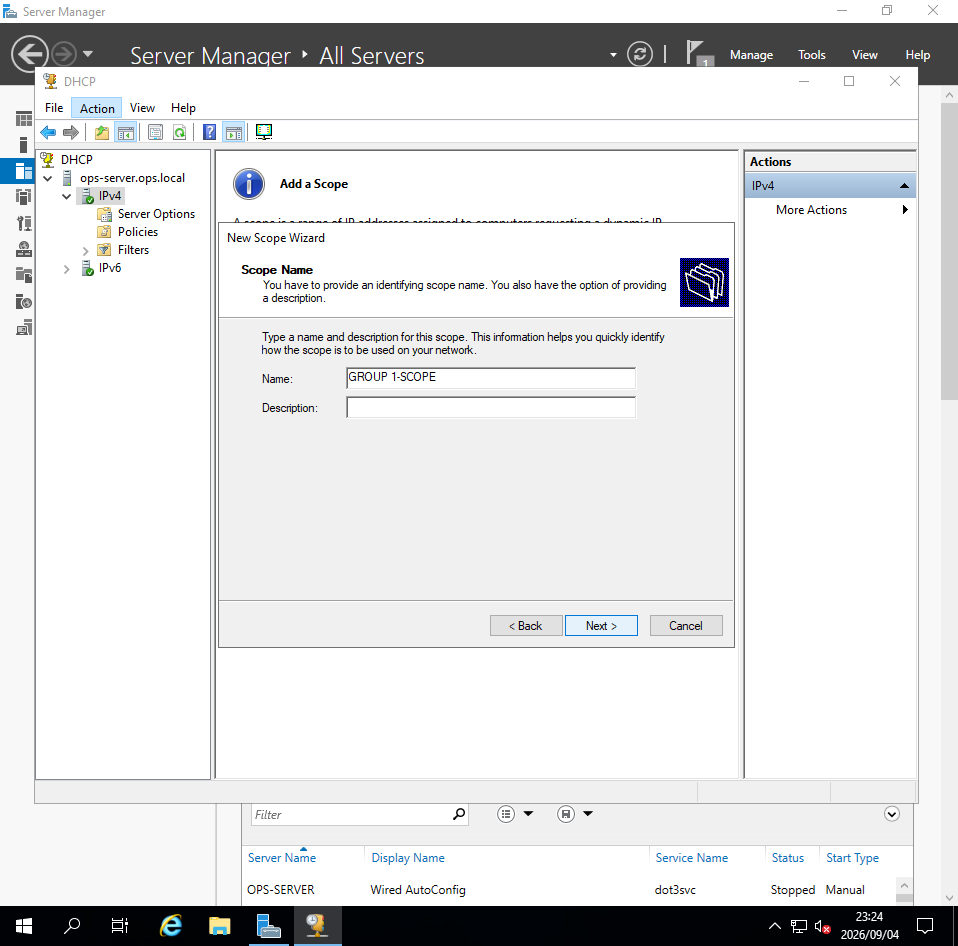
\includegraphics[width=0.7\linewidth]{Images/DHCP/DHCP_08.png}
    \caption{Group One Scope Made}
\end{figure}

\paragraph{}
There exists 4.3 billion posible IPv4 addresses and 3.7 billion available addresses, and therefore,
there exists a countless amount of possible addresses that the scope can allow (\cite{ffIP}).
A scope does not need to accomodate billions of addresses, it just needs a few hundred or a few dozen.
When configuring it, the range of IP addresses needed to be decided.
The addresses that the scope will hand out were from 
192.168.0.100 to 192.168.0.254. This will be the address pool. There were no exclusions 
or delays made in the scope. Alongside handed out IPs, the scope also has
the option to configure the amount of time that a client keeps an assigned IP before renewal, ensuring 
efficient management of IP addresses (\cite{rapidseedbox}). This period of
time is called the lease duration. It was left at the default number of 8 days.

\begin{figure}[H]
    \centering
    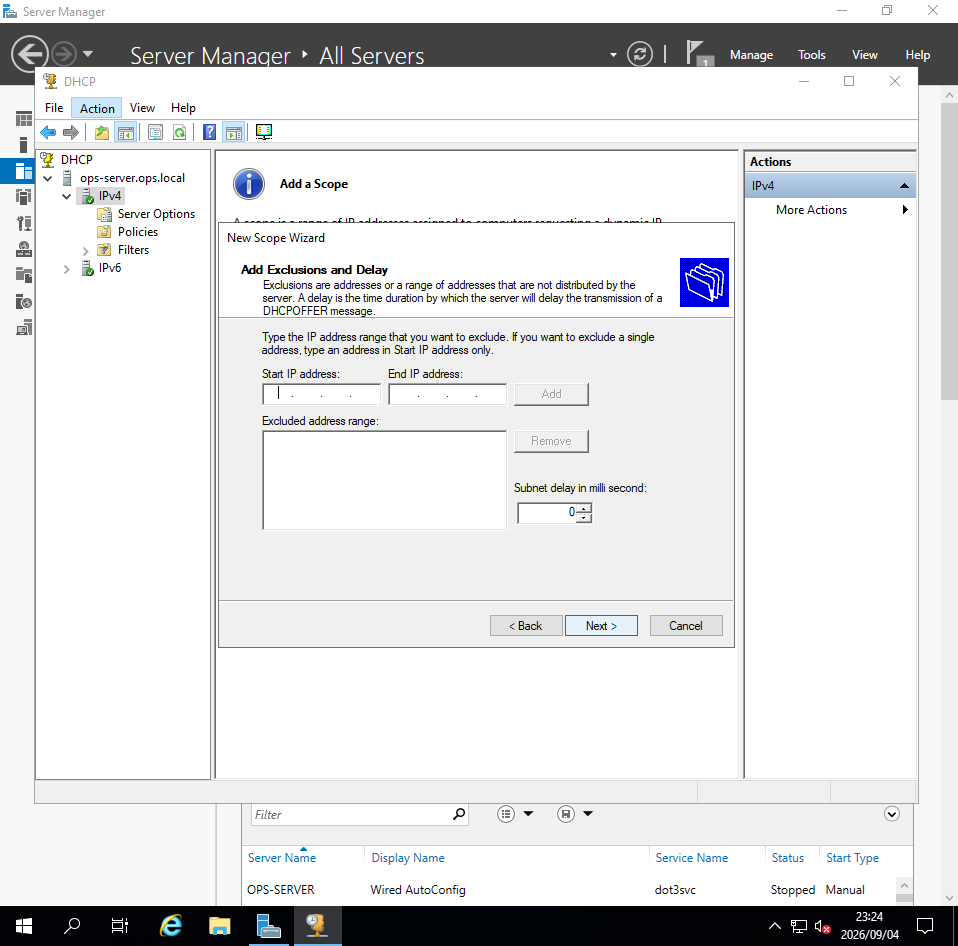
\includegraphics[width=0.7\linewidth]{Images/DHCP/DHCP_10.png}
    \caption{No Exclusions made}
\end{figure}

\begin{figure}[H]
    \centering
    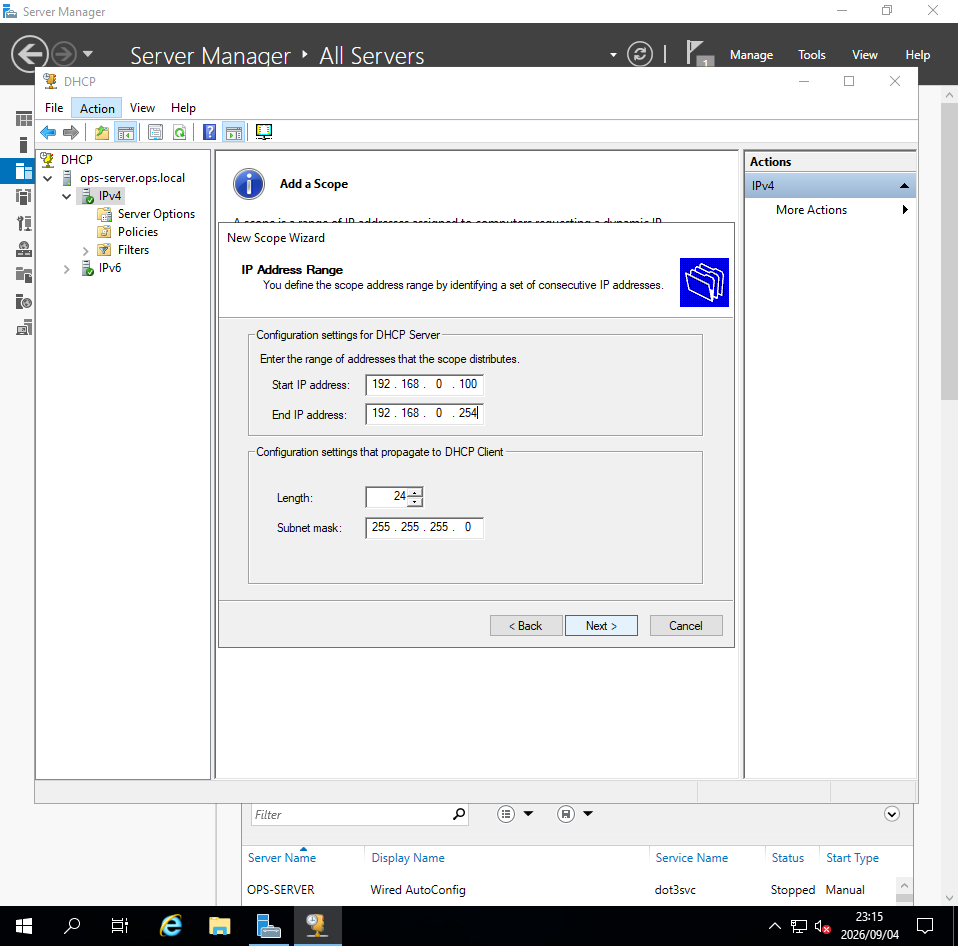
\includegraphics[width=0.7\linewidth]{Images/DHCP/DHCP_09.png}
    \caption{Setting IP Address Range}
\end{figure}

\begin{figure}[H]
    \centering
    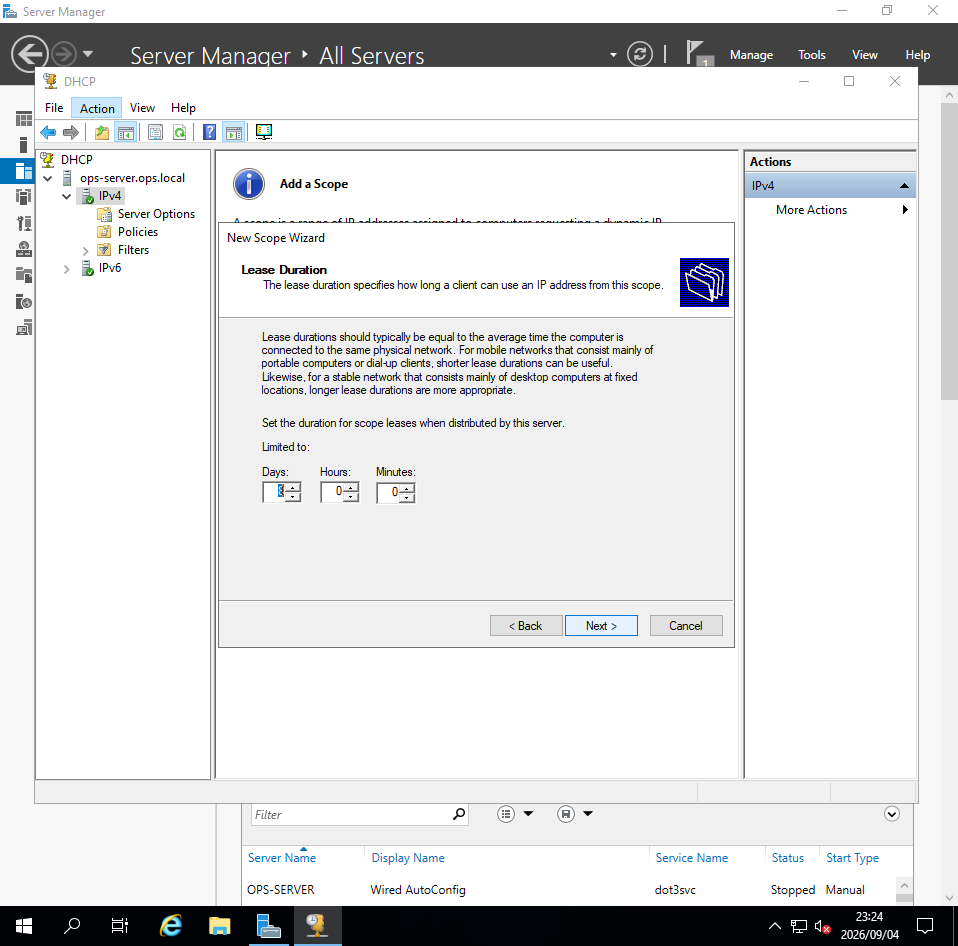
\includegraphics[width=0.7\linewidth]{Images/DHCP/DHCP_11.png}
    \caption{Lease duration of 8 days set}
\end{figure}

\paragraph{}
When clients use the server, access to the internet is an important 
feature that must be present in the server. 
In order for the clients to able to access the internet, 
they need to be able to talk to other devices and networks outside of the DHCP subnet.
A default gateway allows for this. Without it, a client can only reach devices and networks inside 
its own subnet. The default gateway was given the IP address of 192.168.0.1.

\begin{figure}[H]
    \centering
    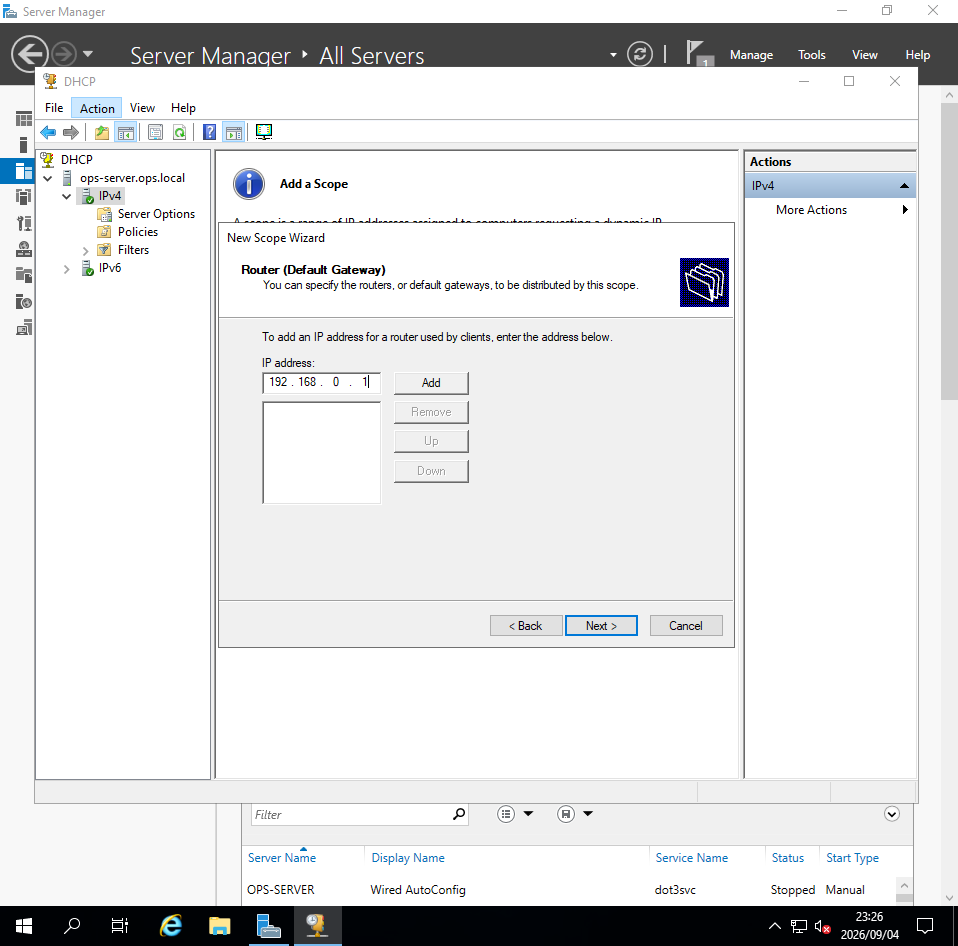
\includegraphics[width=0.7\linewidth]{Images/DHCP/DHCP_12.png}
    \caption{Default Gateway Configured (1)}
\end{figure}

\begin{figure}[H]
    \centering
    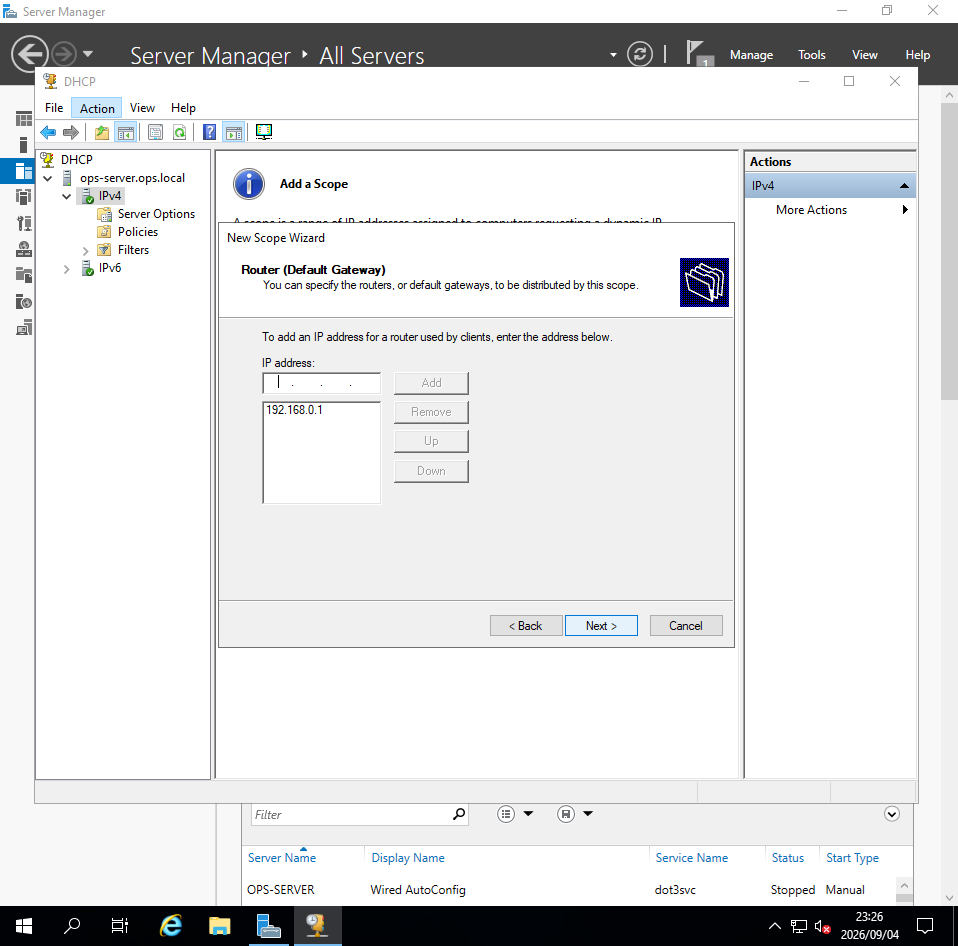
\includegraphics[width=0.7\linewidth]{Images/DHCP/DHCP_13.png}
    \caption{Default Gateway Configured (2)}
\end{figure}

\paragraph{}
After the setting up of the default gateway, the next step was setting up the DNS server.
As mentioned earlier, the DHCP has the job of handing out IP addresses and more for a client to be 
able to use the network. An IP allows a device to communicate with other hosts, but IP addresses 
are inconvinient to memorize or type down. The DNS Server and Domain Name exist 
to allow for devices to access the DHCP server through use of IPs that resolve into domain names (\cite{dns}).
The domain name was set to OPS.local and two IPs, 192.168.0.5 and 8.8.8.8, for two servers were set.
This would mean that in order to access the server they would simply need to type in the domain name, making it 
more accessible for non-domain joined machines.

\begin{figure}[H]
    \centering
    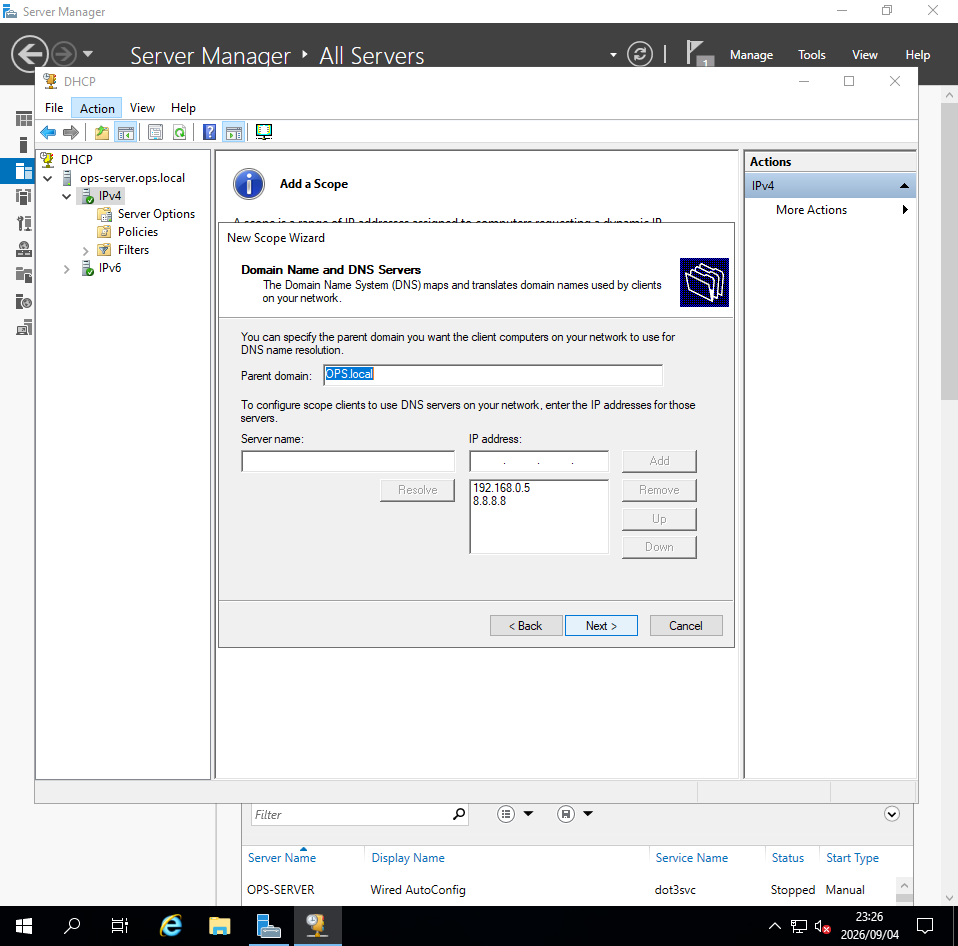
\includegraphics[width=0.7\linewidth]{Images/DHCP/DHCP_14.png}
    \caption{DNS Server and Domain Name}
\end{figure}

\paragraph{}
After the DNS Server and Domain Names are configured, 
there was an option for WINS Server configuration. WINS is a part of the scope 
that resolves NetBOIS computer names to IP Addresses. It is needed to support pre-Windows 2000 
systems and older application using NetBOIS over TCP/IP (\cite{wins}). None of the systems planned to be connected in the network 
do not qualify as pre-Windows 2000 systems, there WINS is not needed.

\begin{figure}[H]
    \centering
    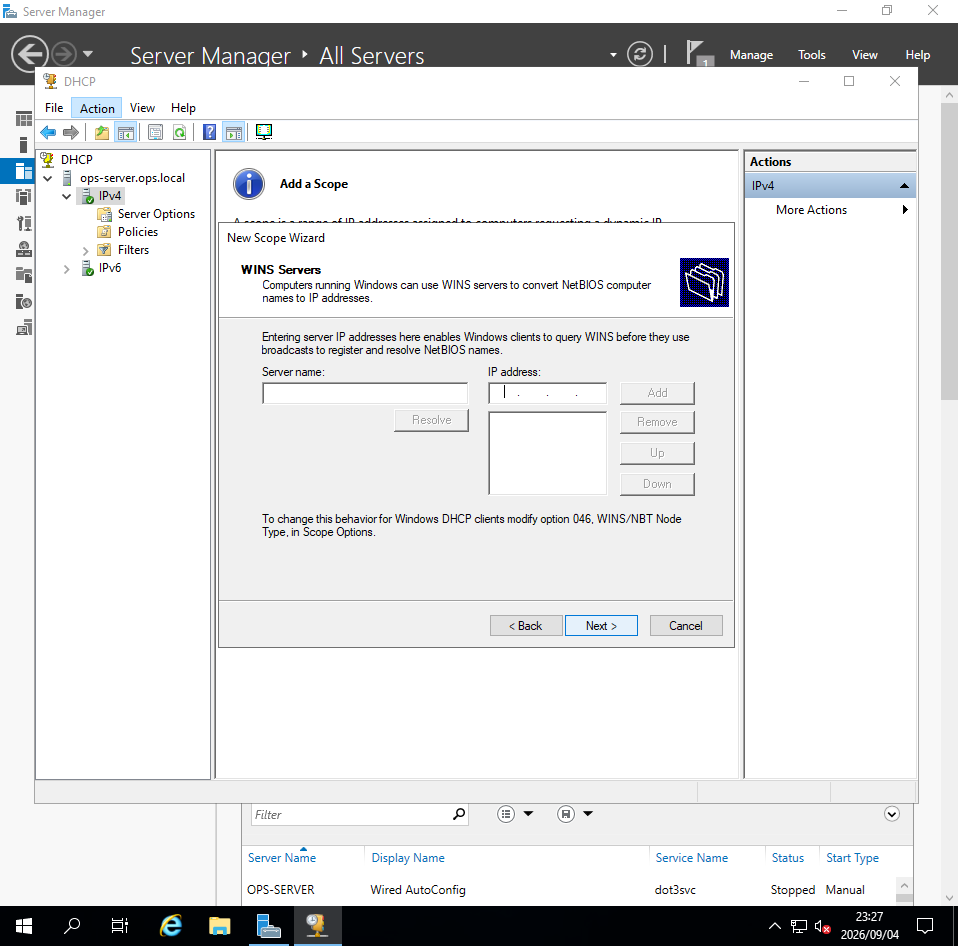
\includegraphics[width=0.7\linewidth]{Images/DHCP/DHCP_15.png}
    \caption{WINS Server configurinf left vacant}
\end{figure}

\paragraph{}
All necessary parts of the scope have been configured. After passing the WINS Server configuring, all that was left was activation of the scope.
Upon activating the scope, the wizard will present completion display. To close the wizard, the finish button was clicked. 
The scope is now activated and ready for testing. The scope will now had out IP addresses from 
192.168.0.100 to 192.168.0.254 and this will be its address pool. At the time of the creation of the scope, 
there were no address leases yet.

\begin{figure}[H]
    \centering
    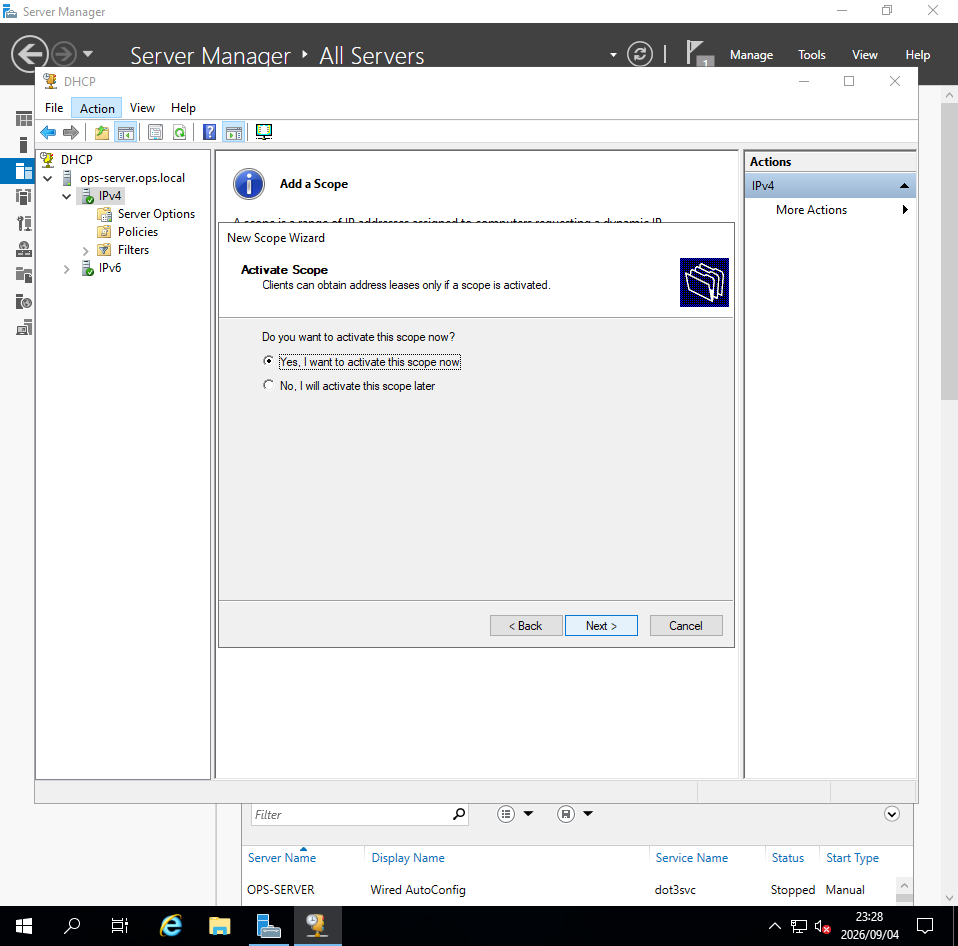
\includegraphics[width=0.7\linewidth]{Images/DHCP/DHCP_16.png}
    \caption{Activation of Scope}
\end{figure}

\begin{figure}[H]
    \centering
    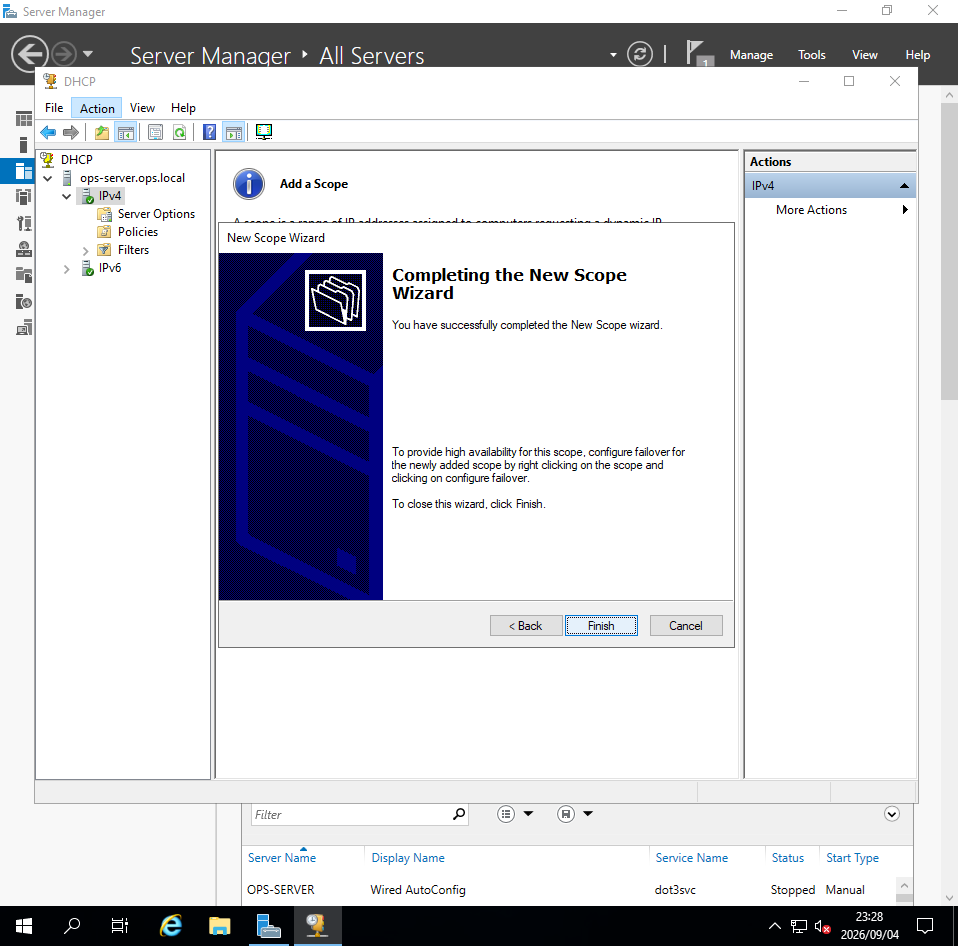
\includegraphics[width=0.7\linewidth]{Images/DHCP/DHCP_17.png}
    \caption{Finishing New Scope Wizard}
\end{figure}
\begin{figure}[H]
    \centering
    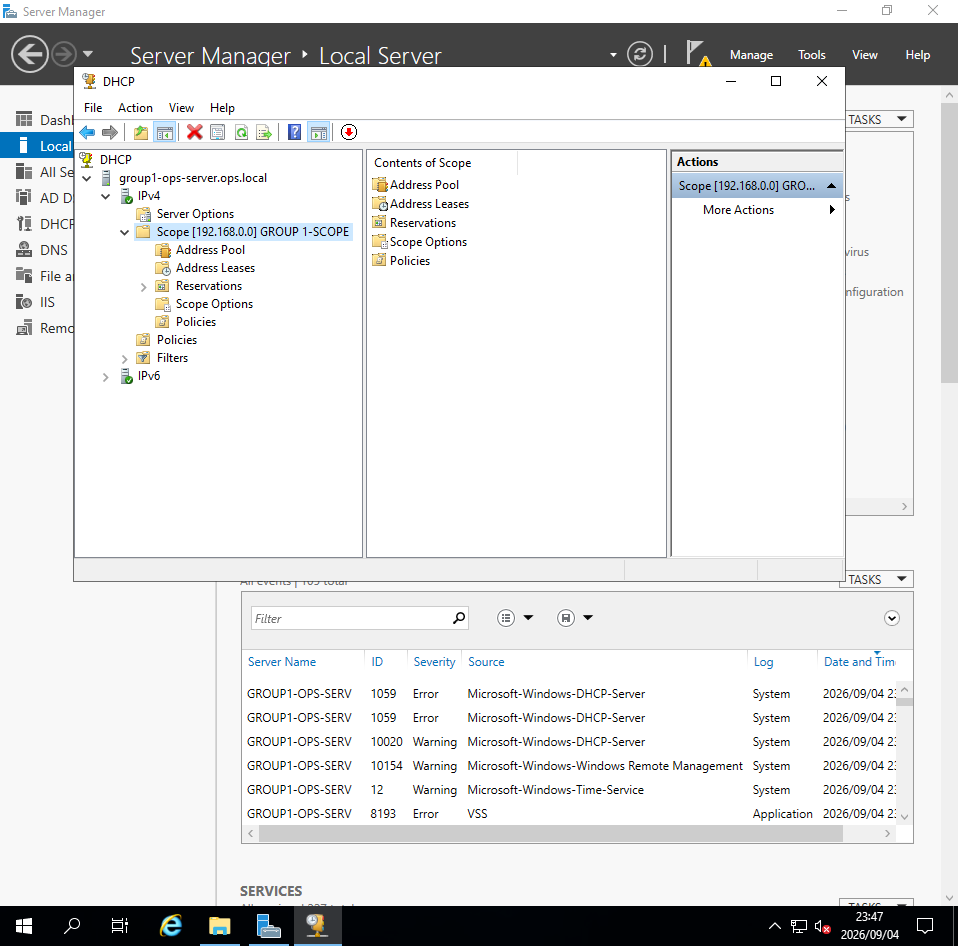
\includegraphics[width=0.7\linewidth]{Images/DHCP/DHCP_18.png}
    \caption{New DHCP Scope created}
\end{figure}

\subsection{Testing of DHCP Server}


DNS Configuration and Testing (20 Marks)

Step One: Verification of DNS Role Installation:

\begin{enumerate}
\def\labelenumi{\arabic{enumi}.}
\item
  Open Server Manager on the server.
\item
  Click the tools icon at the top right hand corner and select DNS.
\item
  Verify that your server appears in the console tree (GROUP1-SVR).
\end{enumerate}

\includegraphics[width=6.01088in,height=3.79942in]{media/image1.png}

Step Two: Configuring the Forward Lookup Zone

2.1. In the DNS Manager expand the GROUP1-SVR node.

2.2. Expand the Forward Lookup Zones.

2.3. Verify that the primary zone has been created for your domain i.e.
Group1.local this will have occurred during the AD DS configuration.

2.4.Click the zone to view the automatically created records (SOA, NS \&
A records).

\includegraphics[width=6in,height=4.13889in]{media/image2.png}

Step Three: Reverse Lookup Zone.

3.1. Right click on the Reverse Lookup Zones and select New Zone.

3.2. Click Next.

3.3. Select Primary zone and make sure Store the zone in Active
Directory is ticked. Hit next.

3.4. Select All DNS servers running on domain controllers in this
domain.

3.5. Select IPv4 Reverse Lookup Zone and hit next.

3.6. Enter your Network ID (i.e. 192.168.64.2) which will be the static
ip address on your Windows Server. Hit next.

3.7. Make sure Only Secure Dynamic Updates are allowed (Recommended for
Active Directory. Hit Finish.

\includegraphics[width=6in,height=3.63889in]{media/image3.png}

Step Four: Adding and Verifying DNS Records.

4.1. Navigate back to your Forward Lookup Zone (Group1cput.local).

4.2. Find your Host (A) record for Group {[}X{]} Windows Server 2019.
Double click to open properties.

4.3. Tick the box stating `Update associated pointer (PTR) record'. Hit
Apply and OK.

4.4. Go to your new Reverse Lookup Zone and refresh. Verify that there
is now a PTR record pointing to your server.

\includegraphics[width=6in,height=3.94444in]{media/image4.png}

Step Five: Testing DNS Resolution (Server \& Client)

Server Side-Test

5.1. Open PowerShell (Or Command Prompt if there are no restrictions on
admins).

5.2. Type `nslookup' and press enter. The Default Server should display
your server name and IP address.

5.3. Perform a forward lookup by entering your servers Fully Qualified
Domain Name (FQDN) (E.g. Group1WindowsServer2019.Group1cput.local) and
pressing enter. You should receive your server IP address.

5.4. Perform a reverse lookup by entering your server IP address (E.g.
192.168.64.2) and pressing enter. You should receive the FQDN.

\includegraphics[width=6in,height=4.68194in]{media/image5.png}

Client Side-Test

5.5. Switch to your client virtual machine running on your Semester 1
Hypervisor. Make sure it is on the same virtual network.

5.6. Open up command prompt/powerShell. Type ping Group1cput.local or
ping your server by name (ping Group1WindowsServer2019).

5.7. Verify that your client can resolve the name to the server IP
address and receive replies.

\includegraphics[width=6in,height=4.76944in]{media/image6.png}

References

McDonald, G., Papadopoulos, P., Pitropakis, N., Ahmad, J., \& Buchanan,
W. J. (2022). Ransomware: Analysing the impact on Windows Active
Directory Domain Services. Sensors, 22, 953. 69

Mokhtar, B., Jurcut, A., ElSayed, M., \& Azer, M. (2022). Active
Directory attacks---Steps, types, and signatures.Electronics , 11, 2629.
41

Moric, Z., Dakic, V., Redzepagic, J., \& Otocan, F. (2024). Penetration
testing and exploitation of Active Directory configuration
vulnerabilities. 2024 4th Intelligent Cybersecurity Conference (ICSC) ,
118-126. 4

Pongsrisomchai, S., \& Ngamsuriyaroj, S. (2019). Automated IT audit of
Windows Server access control. 2019 21st International Conference on
Advanced Communication Technology (ICACT) , 539-544. 1

\chapter{Group Policy setup and configuration for Windows Server 2019}

\section{Introduction}

Group Policy is a feature of Microsoft Windows that provides centralized management and configuration of operating systems, applications, and users' settings in an Active Directory environment. It allows administrators to define security settings, software installation policies, and user interface configurations across multiple computers within a domain.

Well implemented Group Policy can reduce risk, improve security, and ensure consistency across the network. Group Policy Objects (GPOs) can be define for specific users, groups, or computers, and can be linked to organizational units (OUs) to apply settings based on the structure of the Active Directory.

This chapter will cover the setup and configuration of Group Policy in a Windows Server 2019 environment, including the creation of GPOs, linking them to organizational units (OUs), and testing their application.

\section{How does Group Policy work?}

Group Policy relies on the Active Directory infrastructure to apply settings to users and computers. When a user logs in or a computer starts up, the Group Policy engine retrieves the relevant GPOs from the domain controller and applies the settings defined within those GPOs. The order of precedence for applying GPOs is as follows:
\begin{enumerate}
    \item Local Group Policy: Settings defined on the local computer.
    \item Site-level GPOs: Settings defined for the site in which the computer resides.
    \item Domain-level GPOs: Settings defined for the entire domain.
    \item Organizational Unit (OU)-level GPOs: Settings defined for the specific OU in which the user or computer resides. 
\end{enumerate}

When multiple GPOs are applied, the settings from the highest precedence GPO will override those from lower precedence GPOs. This allows administrators to create a hierarchy of policies that can be tailored to specific users, groups, or computers.

Policies are refreshed periodically (every 90 minutes by default), and administrators can also force a Group Policy update using the `gpupdate` command. This ensures that any changes made to GPOs are applied immediately.

\section{Assignment specified Group Policy configuration}

In this scetion we will cover the specific Group Policy configuration required for the assignment. The policies required include disabling command prompt, restricting removable storage access, preventing software installation, and enforcing password complexity requirements. Each of these policies will be configured through the Group Policy Management Console (GPMC) and linked to the appropriate organizational units (OUs) within the Active Directory.

The sections that follows will provide step-by-step instructions for creating and configuring the necessary GPOs, as well as testing their application to ensure they are functioning as intended.

\section{Organizational Unit creation and configuration}

The workflow for creating and configuring Group Policy Objects (GPOs) involves several steps, including accessing the Group Policy Management Console (GPMC), creating a new GPO, configuring the desired settings, and linking the GPO to the appropriate organizational unit (OU). Therefore the OU structure must be defined in Active Directory before creating and linking GPOs.
% OU configuration screenshots
%\screenshot{Images/OU_groups_users/OU_groups_users_01.png}{Active Directory Users and Computers.}{fig:OU_groups_users_01}
%\screenshot{Images/OU_groups_users/OU_groups_users_02.png}{New OU object selected under the domain OPS.local.}{fig:OU_groups_users_02}
%\screenshot{Images/OU_groups_users/OU_groups_users_03.png}{New OU object created and named Group1-OU.}{fig:OU_groups_users_03}
%\screenshot{Images/OU_groups_users/OU_groups_users_04.png}{New OU object listed under the selected domain.}{fig:OU_groups_users_04}
%\screenshot{Images/OU_groups_users/OU_groups_users_05.png}{New User object selected under the Group1-OU.}{fig:OU_groups_users_05}
%\screenshot{Images/OU_groups_users/OU_groups_users_06.png}{New User object configuration.}{fig:OU_groups_users_06}
%\screenshot{Images/OU_groups_users/OU_groups_users_07.png}{New User object password configuration.}{fig:OU_groups_users_07}
%\screenshot{Images/OU_groups_users/OU_groups_users_08.png}{New User object summary.}{fig:OU_groups_users_08}
%\screenshot{Images/OU_groups_users/OU_groups_users_09.png}{User object created and named. Here are two users listed.}{fig:OU_groups_users_09}
%\screenshot{Images/OU_groups_users/OU_groups_users_10.png}{New Group Object selected under the Group1-OU. This allows the grouping of users.}{fig:OU_groups_users_10}
%\screenshot{Images/OU_groups_users/OU_groups_users_11.png}{New Group object configuration. Group name, scope and type configured.}{fig:OU_groups_users_11}
%\screenshot{Images/OU_groups_users/OU_groups_users_12.png}{New Group object listed under the Group1-OU.}{fig:OU_groups_users_12}
%\screenshot{Images/OU_groups_users/OU_groups_users_13.png}{User1 showing membership configuration method 1.}{fig:OU_groups_users_13}
%\screenshot{Images/OU_groups_users/OU_groups_users_14.png}{User1 membership configuration step 1.}{fig:OU_groups_users_14}
%\screenshot{Images/OU_groups_users/OU_groups_users_15.png}{User1 membership configuration step 2.}{fig:OU_groups_users_15}
%\screenshot{Images/OU_groups_users/OU_groups_users_16.png}{User1 membership configuration step 3.}{fig: OU_groups_users_16}
%\screenshot{Images/OU_groups_users/OU_groups_users_17.png}{Group search window}{fig: OU_groups_users_17}
%\screenshot{Images/OU_groups_users/OU_groups_users_18.png}{G1 Users Group find and selection.}{fig:OU_groups_users_18}
%\screenshot{Images/OU_groups_users/OU_groups_users_19.png}{Group selection and addition window.}{fig:OU_groups_users_19}
%\screenshot{Images/OU_groups_users/OU_groups_users_20.png}{User1 membership tab.}{fig:OU_groups_users_20}
%\screenshot{Images/OU_groups_users/OU_groups_users_21.png}{User2 showing membership configuration method 2. Add to a group selected.}{fig:OU_groups_users_21}
%\screenshot{Images/OU_groups_users/OU_groups_users_22.png}{G1 Users Group properties selected to add Users to itself.}{fig:OU_groups_users_22}
%\screenshot{Images/OU_groups_users/OU_groups_users_23.png}{Properties tab with list of members for G1 Users Group.}{fig:OU_groups_users_23}
%\screenshot{Images/OU_groups_users/OU_groups_users_24.png}{Users find and selection.}{fig:OU_groups_users_24}
%\screenshot{Images/OU_groups_users/OU_groups_users_25.png}{User2 selected and will be added to the group.}{fig:OU_groups_users_25}
%\screenshot{Images/OU_groups_users/OU_groups_users_26.png}{Properties tab with list of members for G1 Users Group. The list now includes User2.}{fig:OU_groupsUsers_26}

\section{Group Policy Object creation and configuration}


%\screenshot{Images/GPO/GPO/GPO Cmd 01.png}{Group Policy Management Console. Prevent access to the Command Prompt selected.}{fig:GPO_Cmd_01}
%\screenshot{Images/GPO/GPO/GPO Cmd 02.png}{Policy settings for Prevent access to the Command Prompt. Enabled is selected.}{fig:GPO_Cmd_02}
%\screenshot{Images/GPO/GPO/GPO Cmd 03.png}{Policy settings for Prevent access to the Command Prompt shown as enabled.}{fig:GPO_Cmd_03}
%\screenshot{Images/GPO/GPO/GPO PWD 01.png}{Password Policy settings. Maximum password age selected.}{fig:GPO_PWD_01}
%\screenshot{Images/GPO/GPO/GPO PWD 02.png}{Maximum password age set to 42 days.}{fig:GPO_PWD_02}
%\screenshot{Images/GPO/GPO/GPO PWD 03.png}{Maximum password age shown as 42 days.}{fig:GPO_PWD_03}
%\screenshot{Images/GPO/GPO/GPO PWD 04.png}{Minimum password length set to 10 characters.}{fig:GPO_PWD_04}
%\screenshot{Images/GPO/GPO/GPO PWD 05.png}{Minimum password length shown as 10 characters.}{fig:GPO_PWD_05}
%\screenshot{Images/GPO/GPO/GPO Storage 01.png}{All removable storage classes: Deny all access selected.}{fig:GPO_Storage_01}
%\screenshot{Images/GPO/GPO/GPO Storage 02.png}{All removable storage classes: Deny all access Enabled.}{fig:GPO_Storage_02}
%\screenshot{Images/GPO/GPO/GPO Storage 03.png}{All removable storage classes: Deny all access shown as enabled.}{fig:GPO_Storage_03}
%\screenshot{Images/GPO/GPO/GPO Win Installer 01.png}{Turn off Windows Installer selected.}{fig:GPO_Win_Installer_01}
%\screenshot{Images/GPO/GPO/GPO Win Installer 02.png}{Turn off Windows Installer Enabled.}{fig:GPO_Win_Installer_02}
%\screenshot{Images/GPO/GPO/GPO Win Installer 03.png}{Turn off Windows Installer shown as enabled.}{fig:GPO_Win_Installer_03}

\section{Testing}

Testing is a critical step in the Group Policy configuration process to ensure that the policies are applied correctly and functioning as intended. After creating and linking the GPOs, administrators can use pre-deployment simulation tools to test the policies before applying them in a production environment. Additionally, administrators can use the `gpresult` command to verify that the policies are being applied to the target users and computers. Furthermore, administrators can log in as a user affected by the GPOs to confirm that the restrictions and settings are enforced.
The first and last methods of testing are quiet easily understood and therefore will not be covered in this report. The second method will be covered in the following section.

\section{Chapter Summary}

\ul{Remote Access Setup}

Step One: Adding the role

\begin{enumerate}
\def\labelenumi{\arabic{enumi}.}
\item
  Open up the Server Manager on the main server.
\item
  Click Add Roles and Features. Go through the wizard until you reach
  the Server Roles Tab.
\item
  Click the checkbox next to Remote Access. Press Next until you reach
  the Role Services page.
\item
  Select DirectAccess and VPN (RAS) and Routing. Accept any necessary
  features and press install.
\end{enumerate}

\includegraphics[width=6in,height=4.78681in]{media/image1.png}

Step Two: Configuring RRAS

2.1. Click the Tools section on the Server Manager dashboard and select
Routing and Remote Access.

2.2. Right click on the group server option and select Configure and
Enable Routing and Remote Access.

2.3. Choose Custom configuration or Virtual Private Network (VPN) access
and NAT. Press next.

2.4. Tick the box next to VPN access and press next then Finish. Then
click Start service.

\includegraphics[width=6in,height=4.75in]{media/image2.PNG}

Step 3: User dial-in settings (Active Directory)

3.1. Open the Server Manager. Click on tools and select Active Directory
Users and Computers.

3.2. Create or search for a test user account ie. Group1-SVR.

3.3. Right click on the user account and select Properties. Go to the
Dial-in tab.

3.4. Under Network Access Permission select Allow access. This will
allow the user access to Remote Access permissions.

\includegraphics[width=6in,height=4.76806in]{media/image3.png}

Step 4: Client Testing (Hypervisor)

4.1. On your client virtual machine (semester 1 hypervisor). Navigate to
Network \& Internet Settings. Then click on VPN.

4.2. Click Add a VPN Connection. Select the Windows Built-in VPN
provider. Name it Group 1 VPN. Enter the windows server 2019 machine IP
address.

4.3. Connect to the VPN using the credentials of the user you set up in
step 3.

4.4. Check that the connection has been made. You can do a ping test to
a local resource if needed.

\includegraphics[width=6in,height=4.72917in]{media/image4.PNG}

\include{Chapters/Chapter8_Windows_Certificate}
\chapter{Conclusion}

\section{Summary}

\lipsum

\section{Key Findings}

\lipsum

\section{Future Work}

\lipsum

\section{Final Remarks}

\lipsum

% -------------------------------
% BIBLIOGRAPHY
% -------------------------------
% \printbibliography only prints entries that are actually cited. If you
% still get "Empty bibliography", add \cite{key} in the chapters, or
% temporarily put \nocite{*} on the next line to print every .bib entry.
\clearpage
\addcontentsline{toc}{chapter}{Bibliography}
\printbibliography

% -------------------------------
% APPENDIX
% -------------------------------
\appendix
%To-Do: put in your Appendix
\chapter{Appendix}
\section{Github Repository}


\end{document}